\documentclass[12pt,a4paper]{article}

%\usepackage[UTF8]{ctex}
\usepackage[scale=0.8]{geometry}
\usepackage{amsmath,amsfonts,amssymb,mathrsfs}
\usepackage{abstract,appendix,diagbox,fancyhdr}
\usepackage{makeidx,hyperref}
\usepackage{graphicx,epsfig,subfig}
\usepackage{xcolor}

\newtheorem{theorem}{Theorem}
\newtheorem{remark}{Remark}

\title{Some Results in Anderson Localization}
\author{Chen Jia and Ziqi Liu}
\date{\today}

\begin{document}
\maketitle

\begin{abstract}
In this paper, we focus on two interesting phenomenons in Anderson localization model: phase transition and boundary localization. Under some conditions, the amplitude of quantum states may localize on the boundary. We simulate the boundary localization under various model parameters, and calculate its probability under certain conditions theoretically. The phase transition phenomenone occurs in multi-well potential. We reveal the relationship between the eigenmode degeneracy and the phase transition, and give a concrete method to calculate the value of transition point. Theoretical results are consistent with the simulation.
{\color{red} unfinished...}
\end{abstract}

\section{Introduction}

{\color{red} unfinished...}

\section{Anderson localization under different boundaries}\label{sec:problem}

Anderson localization can be modeled as follows.
\begin{align}\label{eq:eigenproblem}
- \triangle u + V u  = \lambda u \qquad x \in \Omega
\end{align}
The original domain $\Omega = [0,1]^d$ is a d-dimension unit square($d = 1, 2$). In 1-d case, it is divided into $N$ smaller intervals, and $N \times N$ smaller squares in 2-d case. In each interval or square, the potential $V(x)$ is constant. Its value on each part is determined randomly between $0$ and $K$. The eigenfunction $u(x)$ and eigenvalue $\lambda$ represents the eigenmodes and energy levels of the Hamiltonian.

Boundary conditions (BC) of the model can be choosen as Dirichlet
\begin{align}\label{eq:Dirichlet}
u|_{\partial \Omega} = 0
\end{align}
Neumann
\begin{align}\label{eq:Neumann}
\frac{\partial u}{\partial \mathbf{n}}|_{\partial \Omega} = 0
\end{align}
Robin($h > 0$)
\begin{align}\label{eq:Robin}
(\frac{\partial u}{\partial \mathbf{n}} + h u)|_{\partial \Omega} = 0
\end{align}
or parabolic boundary condition.

Most works focus on Dirichlet boundary condition, but we would indicate that eigenmodes and eigenvalues may perform differently under different boundary conditions. As shown in Figure \ref{fig:4}, under Dirichlet and Neumann BC, difference of eigenmode is obvious, but egienvalues not. For larger eigenvalues, difference of eigenmodes are much larger.
\begin{figure}[h]
\centering
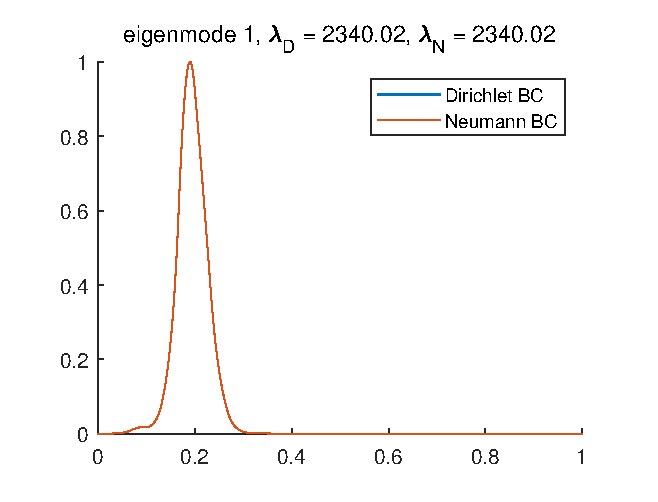
\includegraphics[width=0.24\linewidth]{F4E1}
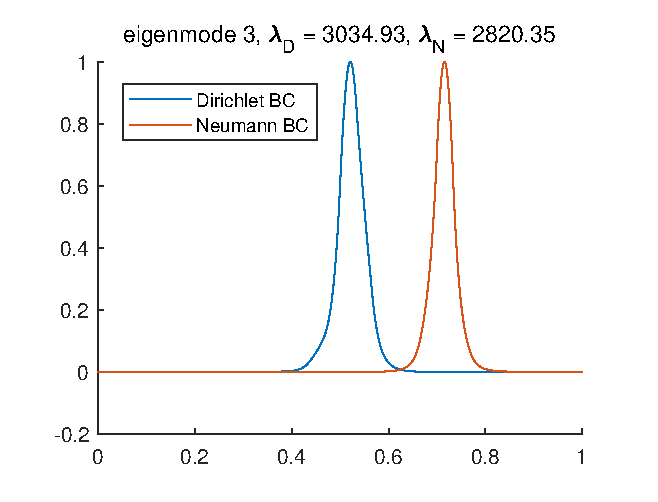
\includegraphics[width=0.24\linewidth]{F4E3}
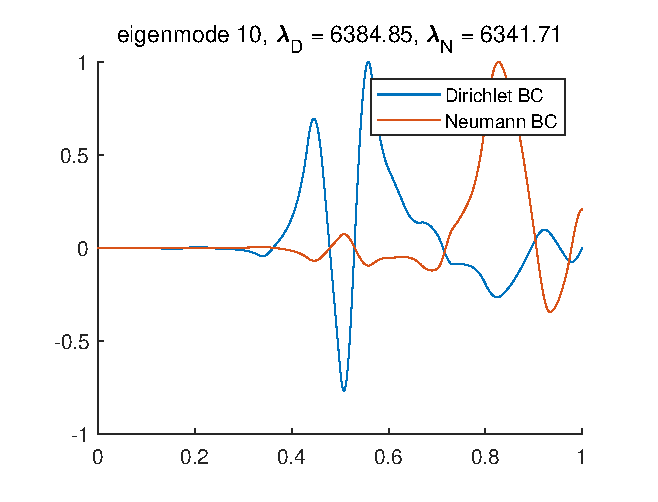
\includegraphics[width=0.24\linewidth]{F4E10}
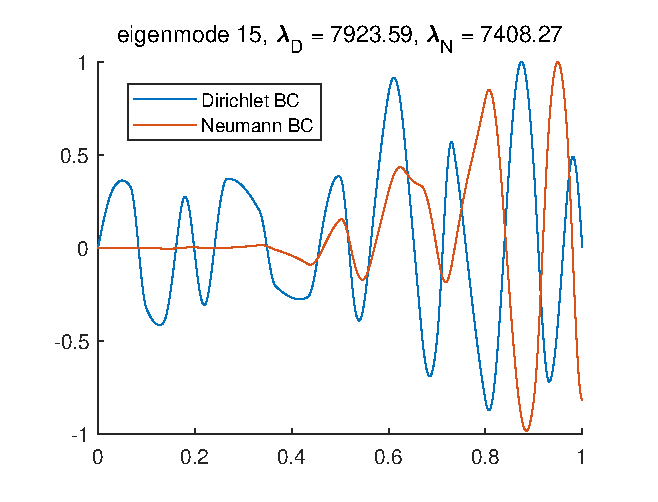
\includegraphics[width=0.24\linewidth]{F4E15}
\caption{Eigenmodes and eigenvalues (1-d case) under Dirichlet BC (blue lines) and Neumann BC (red lines)}
\label{fig:4}
\end{figure}

Figure \ref{fig:5} shows the 2-d case. It's intersting that both eigenvalues and eigenmodes are totally different in 2-d case. 

\begin{figure}[h]
\centering
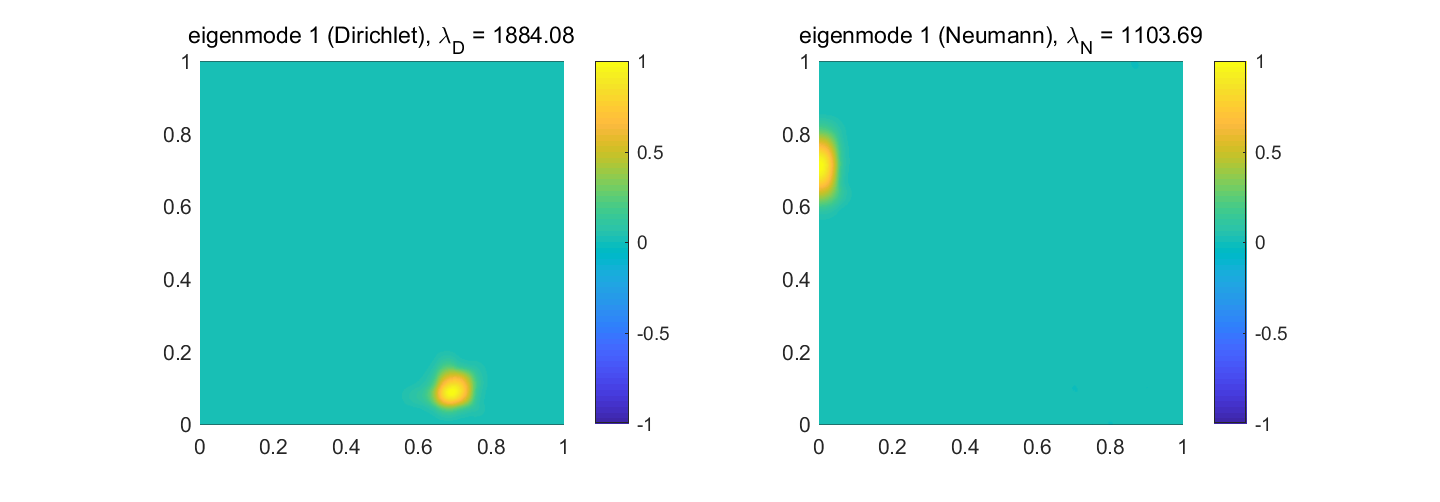
\includegraphics[width=0.45\linewidth]{F5E1}
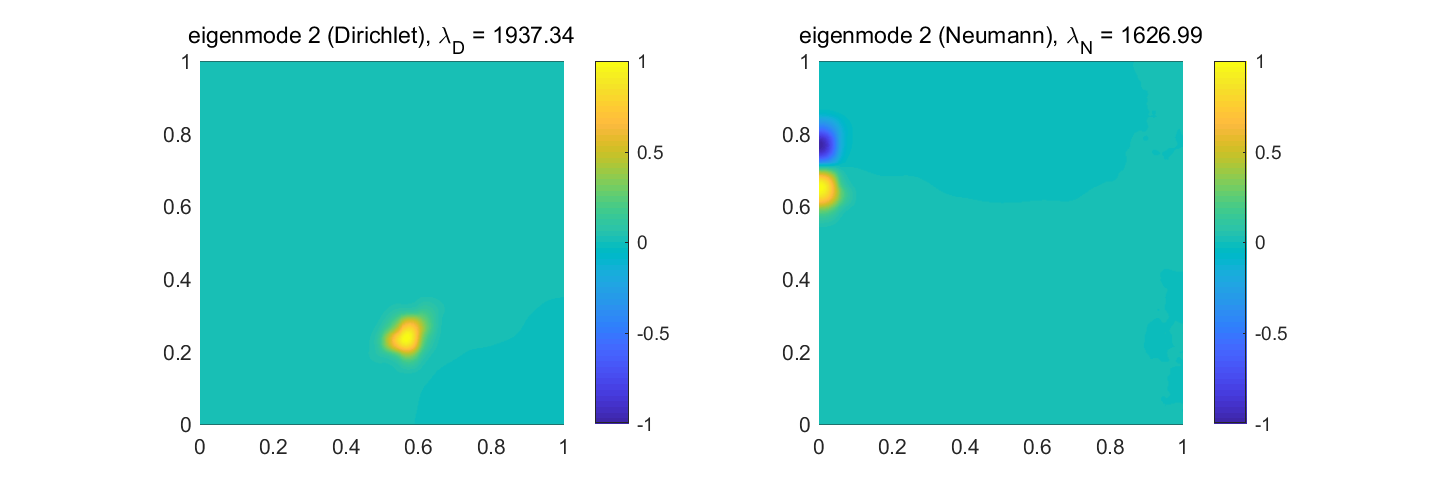
\includegraphics[width=0.45\linewidth]{F5E2}
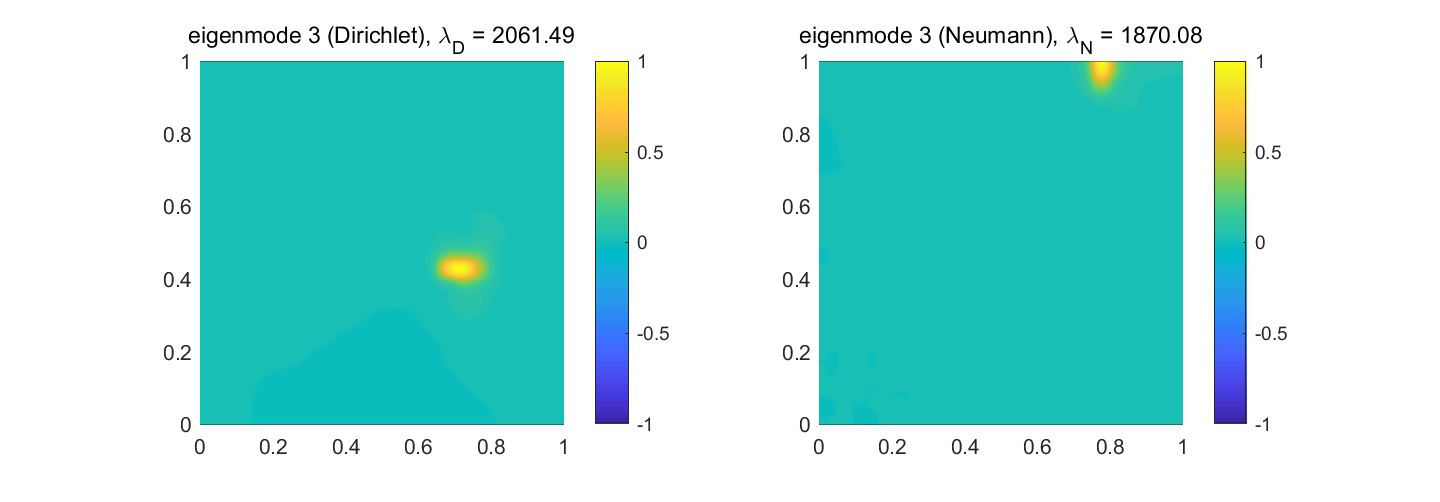
\includegraphics[width=0.45\linewidth]{F5E3}
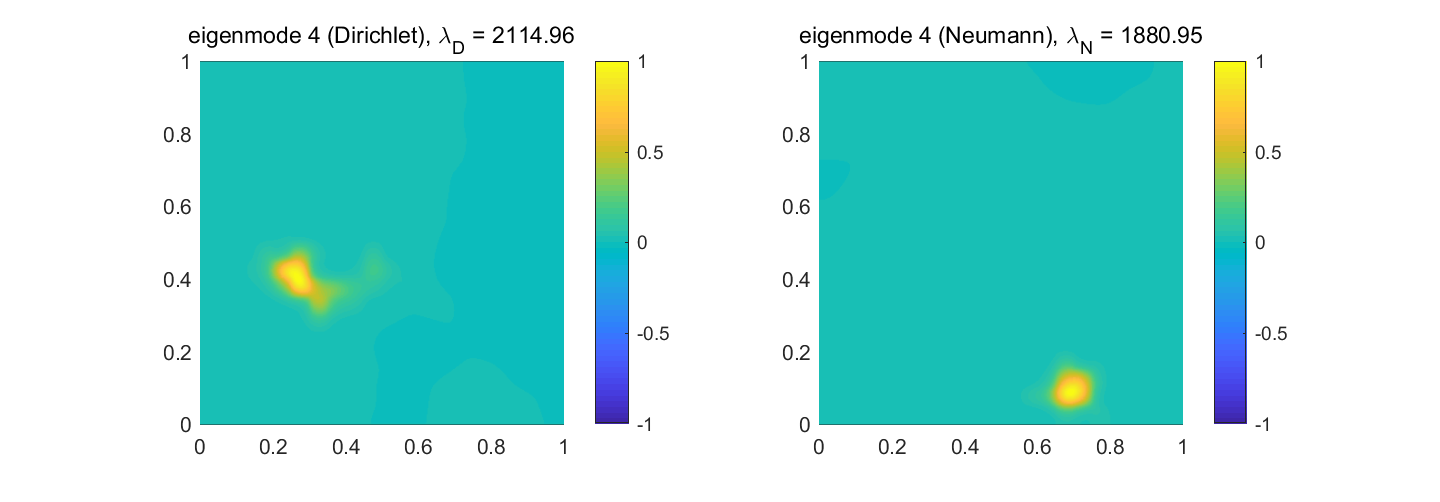
\includegraphics[width=0.45\linewidth]{F5E4}
\caption{First 4 eigenmodes and eigenvalues (2-d case) under Dirichlet BC (left of each subfigure) and Neumann BC (right of each subfigure)}
\label{fig:5}
\end{figure}

Eigenvalues under different boundary conditions performs differently in 1-d and 2-d case. Figure \ref{fig:45} shows the difference in respect of increasing rates.
\begin{figure}[h]
\centering
\subfloat[1-d case]{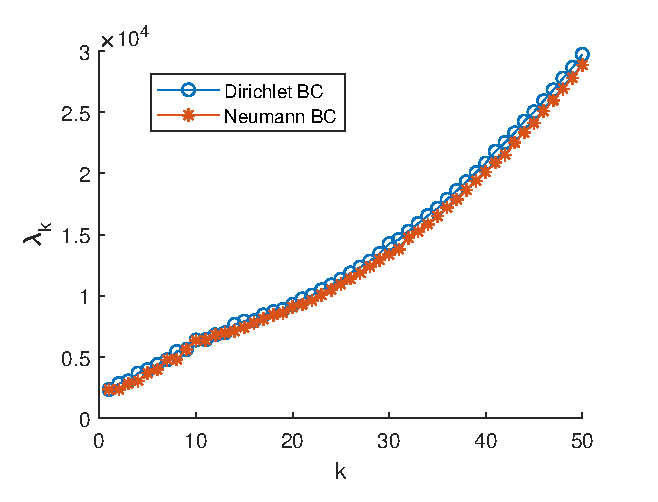
\includegraphics[width=0.33\linewidth]{F4L}}
\subfloat[2-d case]{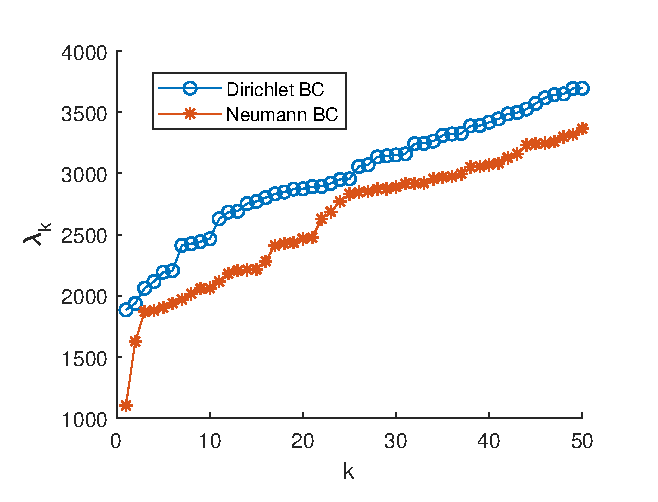
\includegraphics[width=0.33\linewidth]{F5L}}
\caption{Difference of eigenvalues between 1-d and 2-d case. x-axis represents the serial number $k$ of eigenvalues and y-axis represents the correspoing eigenvalue $\lambda_k$}
\label{fig:45}
\end{figure}

We can see that under Dirichlet BC, eigenmodes can not localize to the boundary due to the enforce boundary condition, but under other boundary conditons, eigenmodes may localize to the boundary. It is one of mean results in this papper. Porbility of localization on boundary is discussed in Section \ref{sec:probability}.

{\color{gray} boundary condition is important in model, our work make sense.}

\section{Landscape of localization}\label{sec:landscape}

\subsection{basic theroies}

We compute the eigenmodes in 1-d case under different boundary conditions. Eigenmodes are normalized as $\|u\|_{\infty} = 1$. Random potential $V(x)$ and the eigenmodes $u(x) / \lambda$ (colored lines) are shown in Figure \ref{fig:1}. It seems diffcult for us to predict where the eigenmode will localize before simulation.

In order to predict where will eigenmodes localize, we introduce the landscape $w(x)$ as the sulotion of the right hand side equation with the same boundary condition.
\begin{align}\label{eq:landscape}
- \triangle w + V w  = 1 \qquad x \in \Omega
\end{align}
In Figure \ref{fig:1}, landscape is shown by black lines. Noting that eigenmodes and landscaps behave differently under different boundary conditions.

\begin{figure}[h]
\centering
\subfloat[potential]{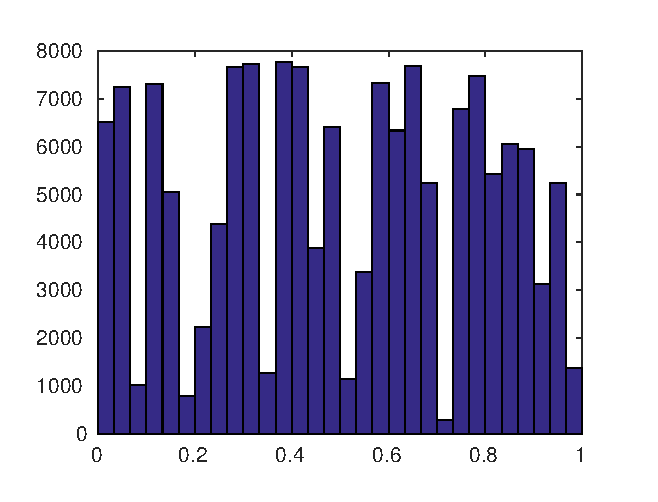
\includegraphics[width=0.24\linewidth]{F1V}}
\subfloat[Dirichlet]{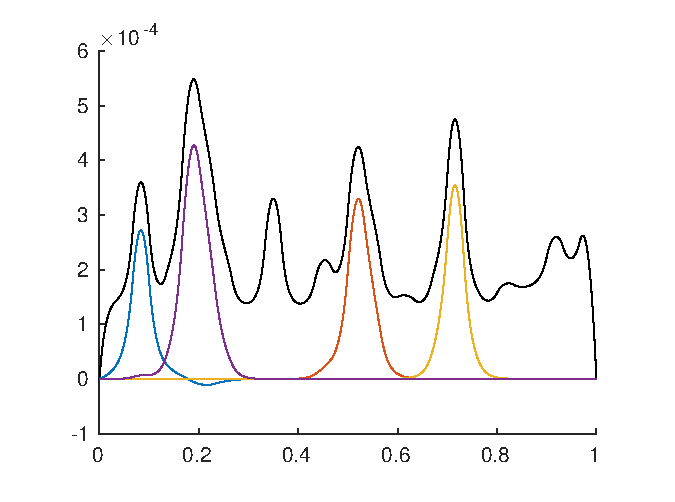
\includegraphics[width=0.24\linewidth]{F1D}}
\subfloat[Neumann]{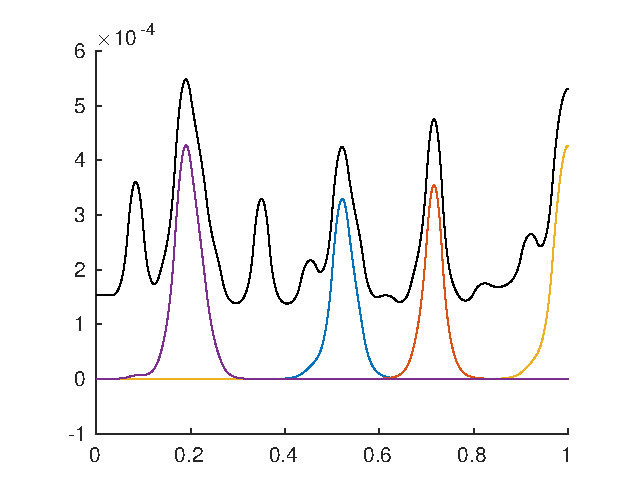
\includegraphics[width=0.24\linewidth]{F1N}}
\subfloat[Robin]{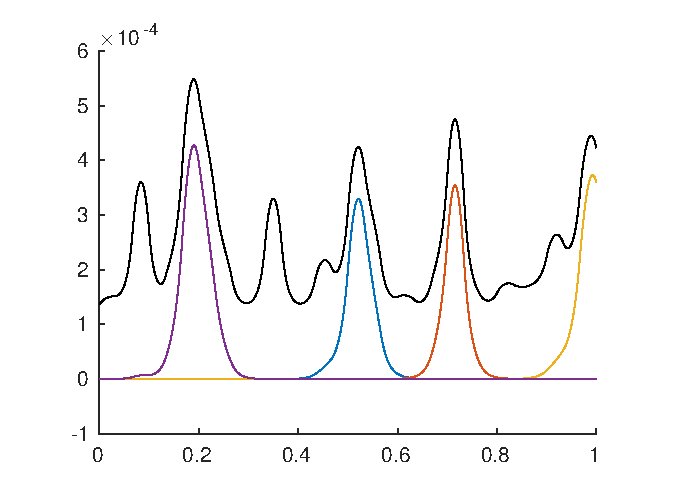
\includegraphics[width=0.24\linewidth]{F1R}}
\caption{(a) The random potential $V(x)$ entering the equation(we choose $K = 5000$). The domain $[0,1]$ is divided in $N = 30$ smaller intervals. (b-d) First 4 eigenmodes $u(x) / \lambda$ (colored lines) and landscape $w(x)$ (black line) under certian potential. eigenmodes and landscapes are computed under Dirichlet, Neumann, Robin ($h = 10$) BC.}
\label{fig:1}
\end{figure}

In simulation, we can see that eigenmodes satisify $u(x) / \lambda \leq w(x)$, actually we have following therom.

\begin{theorem}\label{th:landscape}
Domain $\Omega \subset \mathbb{R}^d$ is an open bounded set. Consider $\lambda \in \mathbb{R}$ and $u(x)$ are one of the eigenvalue and corresponding eigenfunction of the second order elliptic problem
\begin{align}
-\nabla(A \nabla u) + b \cdot \nabla u + c u = \lambda u \qquad x \in \Omega
\end{align}
whose boundary condition can be Dirichlet, Neumann, Robin($h > 0$) and parabolic, $A(x)$ is positive define and $c(x) \leq 0$. $u(x)$ is normalized as $\|u\|_{\infty} = 1$.

Landscape $w(x)$ is the sulotion of this equation with the same boundary condition.
\begin{align}
-\nabla(A \nabla w) + b \cdot \nabla w + c w = 1 \qquad x \in \Omega
\end{align}

Then we have
\begin{align}\label{eq:control}
u(x) \leq \lambda \, w(x) \qquad x \in \Omega
\end{align}
\end{theorem}

\begin{remark}
The idea of landscape first appeared in \cite{pnas}, but only the simplest case (Dirichlet BC + symetric operator) is strictly proofed. We expand the theory to the more general non-symetric operator and arbitrary boundries.
\end{remark}

\subsection{valleylines and effective valleylines for 2-d case}

When we come to 2-d case, landscape becomes more complex. We divied the peaks of landscape by valleylines which can be calculated by applying watershed algorithm to the reversed landscape. Along the valleylines, $w(x)$ is expected to be small. Valley lines divide the hole domain into many sub-domains, according to the therom \ref{th:landscape}, $u(x)$ is also small on the valleylines, so eigenmodes are likely to localize in these sub-domains.

Figure \ref{fig:2} shows the landscape, eigenmodes and valleylines under Neumann boundary condition. If we only consider the landscape in (b), we can hardly get the sketch of eigenmodes, but in (d), valleylines seperate the eigenmodes properly.

\begin{figure}[h]
\centering
\subfloat[potential]{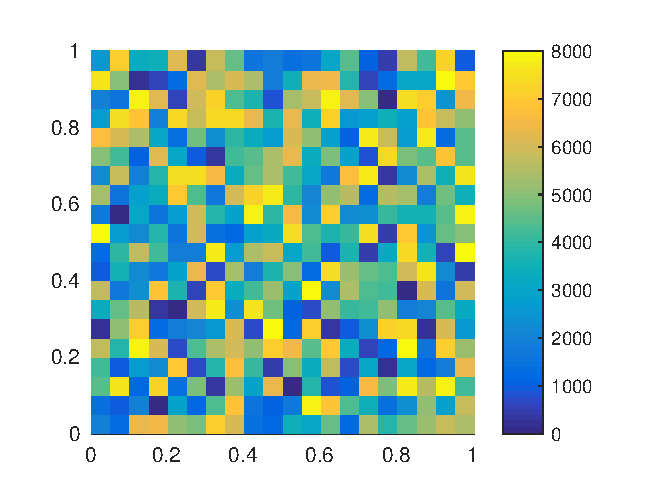
\includegraphics[width=0.24\linewidth]{F2P}}
\subfloat[landscape]{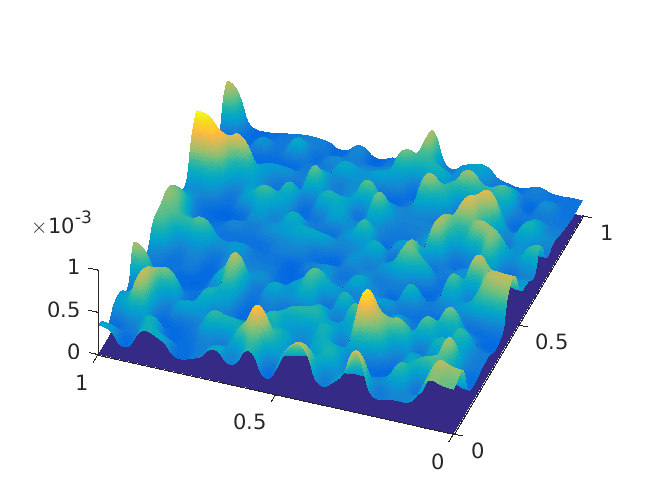
\includegraphics[width=0.24\linewidth]{F2W}}
\subfloat[valleylines]{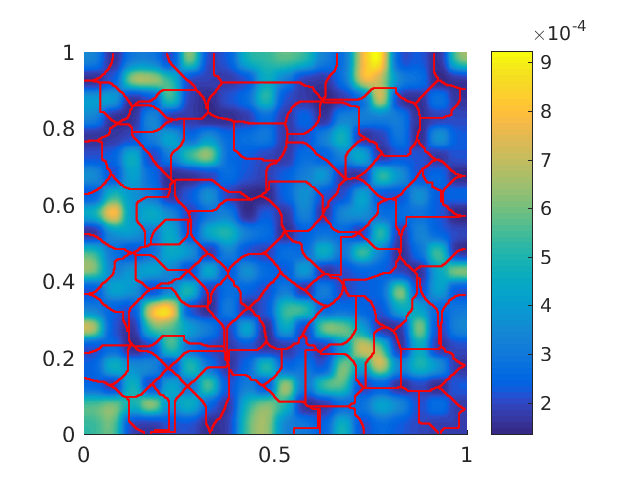
\includegraphics[width=0.24\linewidth]{F2V}}
\subfloat[eigenmodes]{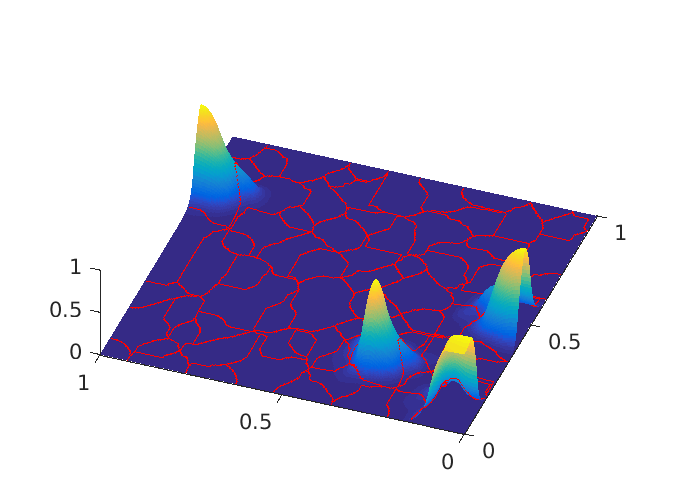
\includegraphics[width=0.24\linewidth]{F2E}}
\caption{(a) The random potential $V(x)$ entering the equation($K = 8000$). The domain $[0,1]^2$ is divided in $20 \times 20$ smaller squares. (b) 3-d view of landscape $w(x)$ under the potential and Neumann BC. (c) 2-d color representation of $w(x)$ and valleylines deduced from the landscape (red lines). (d) first 4 eigenmodes and valleylines.}
\label{fig:2}
\end{figure}


For larger eigenvalues, since $\lambda$ may be big, some parts of valleylines may lose their control on eigenmodes. That is, only the points on valleylines satisify $w(x) < 1$ is effective. We calculate larger eigenmodes and efective valleylines, shown in Figure \ref{fig:3}. One can clearly observe that all modes are localized in one of the subregions divided by effective valleylines.

\begin{figure}[h]
\centering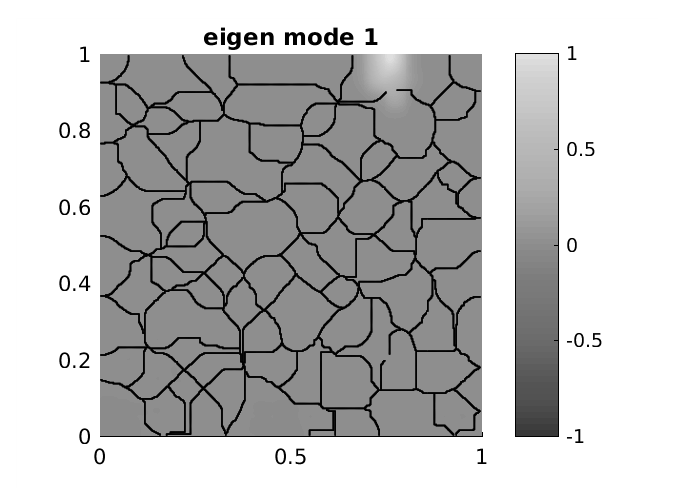
\includegraphics[width=0.24\linewidth]{F3E1}
\centering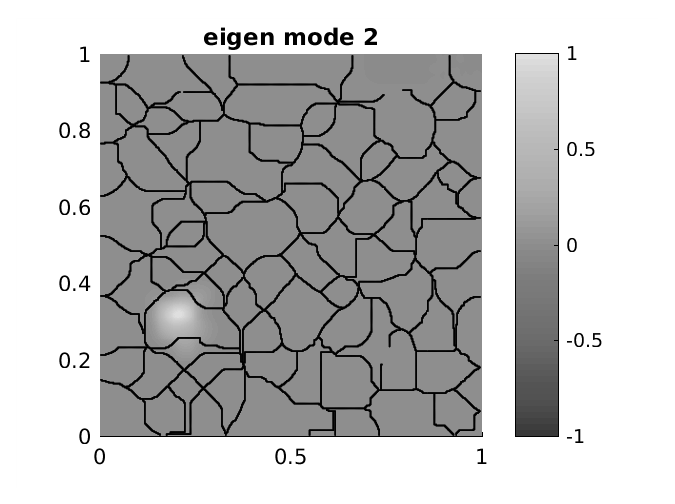
\includegraphics[width=0.24\linewidth]{F3E2}
\centering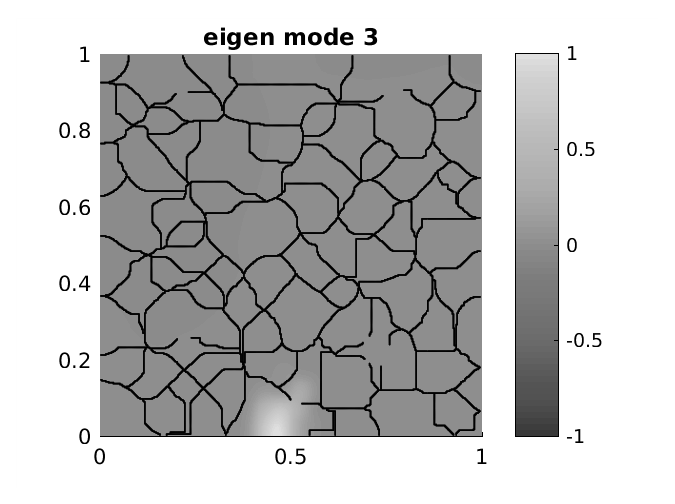
\includegraphics[width=0.24\linewidth]{F3E3}
\centering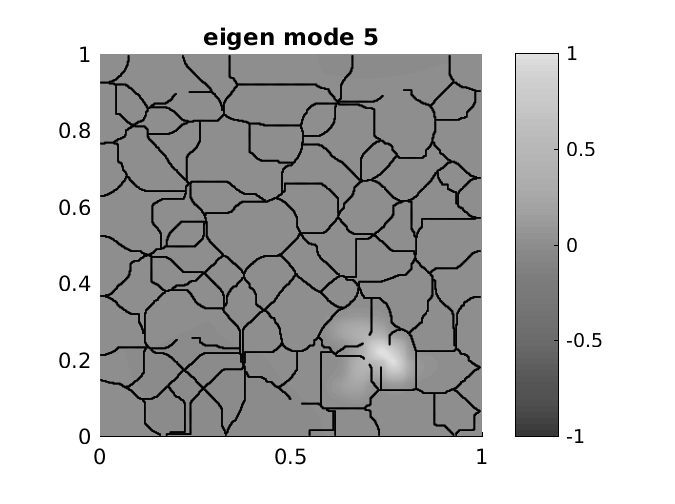
\includegraphics[width=0.24\linewidth]{F3E5}
\centering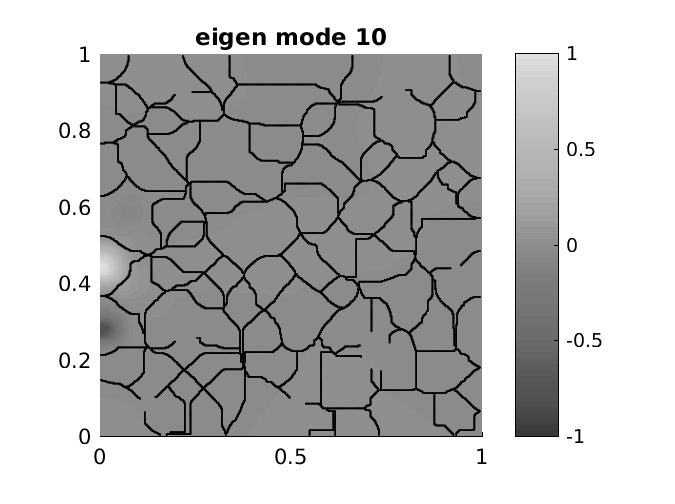
\includegraphics[width=0.24\linewidth]{F3E10}
\centering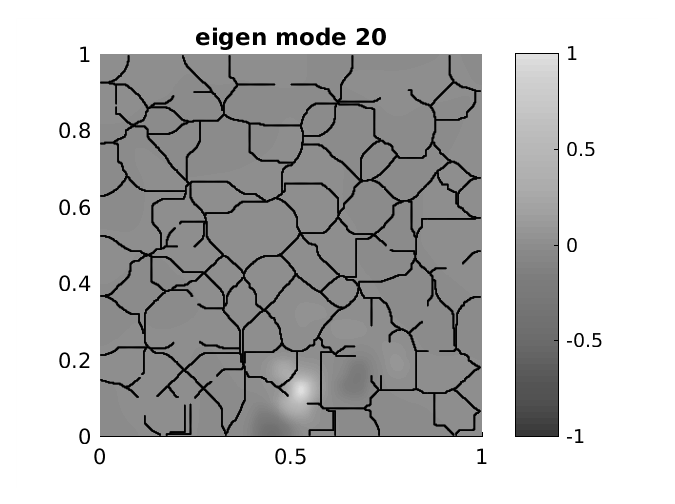
\includegraphics[width=0.24\linewidth]{F3E20}
\centering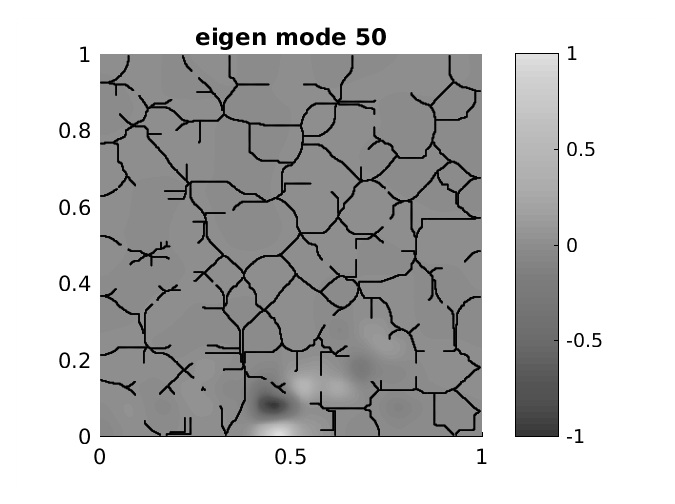
\includegraphics[width=0.24\linewidth]{F3E50}
\centering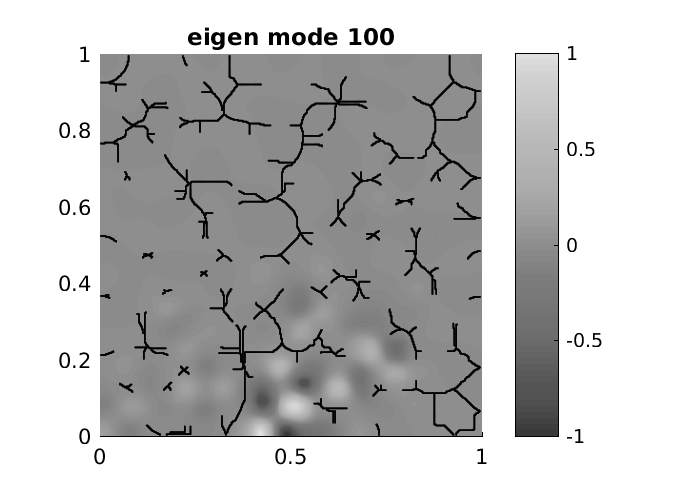
\includegraphics[width=0.24\linewidth]{F3E100}
\caption{Eigenmodes and corresponding effecitve valleylines (black lines)}
\label{fig:3}
\end{figure}

\section{Limit Behavior under large K}\label{sec:limit}

In following sections, we consider the case that $V(x)$ in each interval or square corresponds Bernoulli distribution. That is, in each subdomain, potential is $0$ with probability $1-p$ and $K$ with probability $p$.

In this case, we have the following therom.
\begin{theorem}\label{th:largeK}
Domain $\Omega \subset \mathbb{R}^d$ is an open bounded set. Consider $\lambda \in \mathbb{R}$ and $u(x)$ are one of the eigenvalue and corresponding eigenfunction of the problem \ref{eq:eigenproblem}. $V(x) \in \{0, K\} \ \forall \, x$ and $u(x)$ is normalized as $\|u\|_{\infty} = 1$.

Then for the subdomian $D = \{x \in \Omega: V(x) = K\}$we have
\begin{align}\label{eq:largeK}
\lim_{K \rightarrow \infty} u(x) = 0 \qquad \forall x \in D
\end{align}
\end{theorem}

According to the theorem, the original problem turns to some eigenvalue problems on subdomains where $V(x)$ is $0$. The first eigenmode will licalize to the subdomain with smallest eigenvalue.

In 1-d case, the result is trival, we focous on the 2-d case. Figure \ref{fig:7} shows the potentials and valleylines for $p = 0.7$ with different $K$. With the increasing of $K$, the subdomains divided by valleylines split and finally coincides with the connected branches of $V(x) = 0$. Figure \ref{fig:6} shows the potentials and valleylines of $K = 10^4$, the valleylines surrounds the connected branch of $V(x) = 0$, and avoids crossing the parts of $V(x) = K$ as far as possible.

\begin{figure}[h]
\centering
\subfloat[$K=10$]{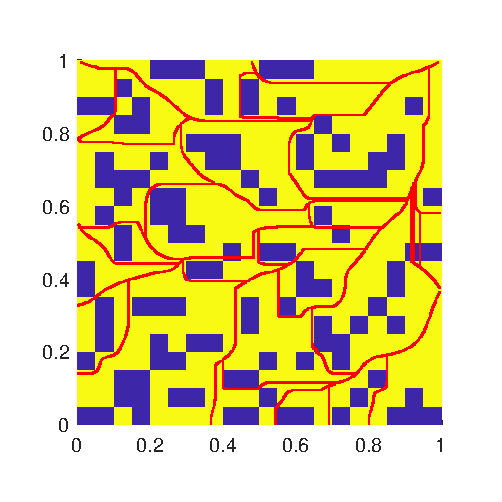
\includegraphics[width=0.33\linewidth]{F7K1}}
\subfloat[$K=100$]{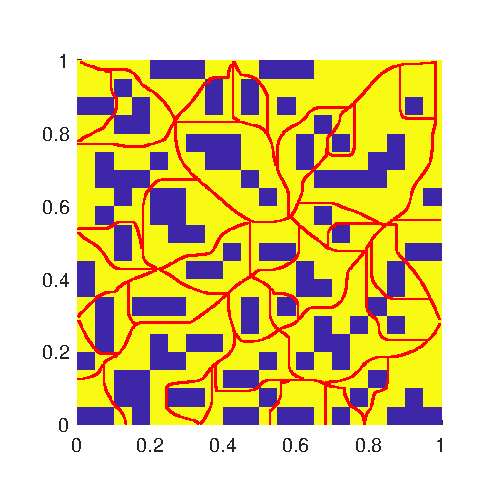
\includegraphics[width=0.33\linewidth]{F7K2}}
\subfloat[$K=1000$]{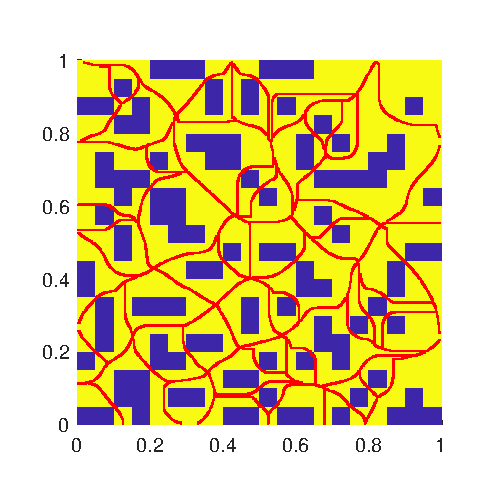
\includegraphics[width=0.33\linewidth]{F7K3}}
\caption{Potentials (blue for $V(x) = 0$ and yellow for $V(x) = K$) and valleylines (red lines) for different $K$}
\label{fig:7}
\end{figure}

\begin{figure}[h]
\centering
\subfloat[$p=0.5$]{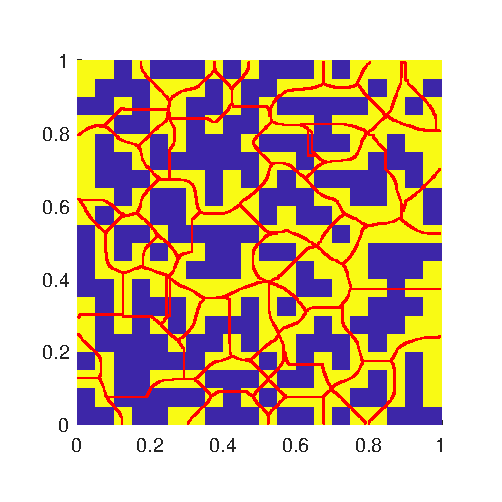
\includegraphics[width=0.33\linewidth]{F6P5}}
\subfloat[$p=0.7$]{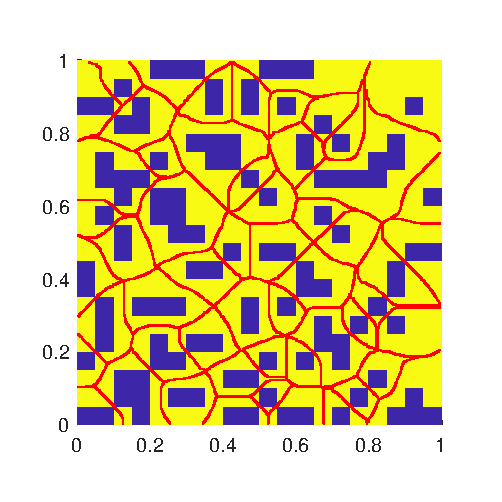
\includegraphics[width=0.33\linewidth]{F6P7}}
\subfloat[$p=0.9$]{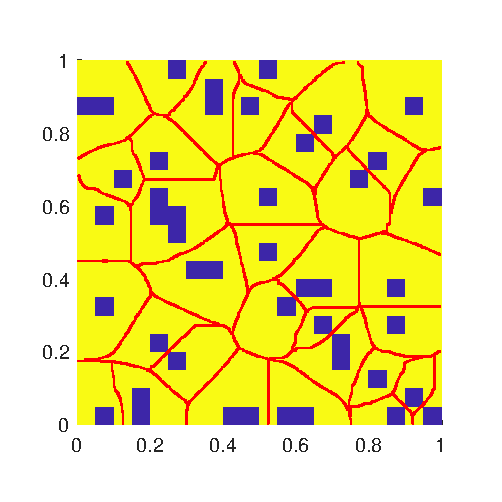
\includegraphics[width=0.33\linewidth]{F6P9}}
\caption{Potentials (blue for $V(x) = 0$ and yellow for $V(x) = K$) and valleylines (red lines) for $K = 10^4$}
\label{fig:6}
\end{figure}

\section{Localization to the boundary}\label{sec:probability}

In Section \ref{sec:landscape}, we indicate that eigenmodes may localize to the boundary in Neumann and Robin BC. In this section, we will discuss the probability of localization to the boundary theoretically under specific conditions.

In the 1-d case, for a certain eigenmode, the degree of its localization to the boundary is defined as
\begin{align}
P_b = \frac{\max\{|u(0)|, |u(1)|\}}{\max_{x \in \Omega} |u(x)|}
\end{align}

In 2-d case, we can define the degree of localization to the edge as
\begin{align}
P_e = \frac{\max_{x \in \partial\Omega} |u(x)|}{\max_{x \in \Omega} |u(x)|}
\end{align}
and the degree of localization to the corner as
\begin{align}
P_c = \frac{\max\{|u(0,0)|, |u(0,1)|, |u(1,1)|, |u(1,0)|\}}{\max_{x \in \Omega} |u(x)|}
\end{align}

Under Dirichlet BC, $P_b$, $P_e$ and $P_c$ are constantly $0$, but under Neumann and Robin BC, these are random varaibles related on $K$, $p$ and $h$. For simplicity, we focous on only the first eigenmode.

In following simulation, for 1-d case, hole domain $[0,1]$ is divided into $50$ small intervals, for 2-d case, $[0,1]^2$ is divided into $15 \times 15$ small squares. We randomly generate the potential $1000$ times to get the mean value of $P_b$, $P_e$ and $P_c$.

\subsection{some simulation results}

\paragraph{relation of parameter h}

The degree of localization to the boundary varies to $h$ with parameter $p=0.5, K=10^3$ is shown in the Figure \ref{fig:8h}. In Robin BC, when $h$ goes to infinity, the boundary approches Dirichlet, and when $h$ goes to $0$, the boundary approches Neumann.

\begin{figure}[h]
\centering
\subfloat[boundary]{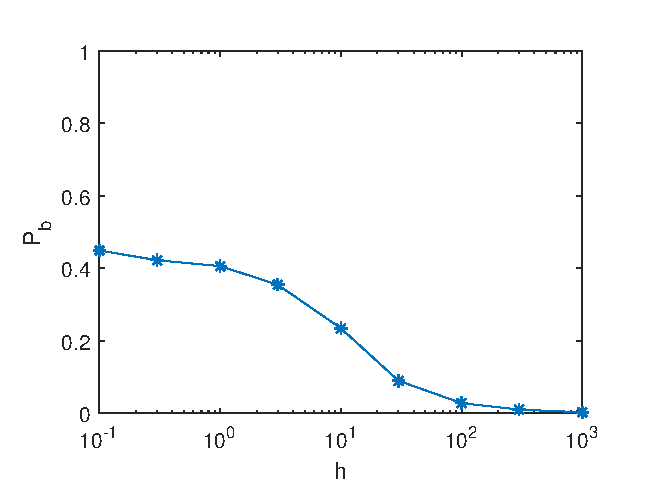
\includegraphics[width=0.33\linewidth]{F8hb}}
\subfloat[edge]{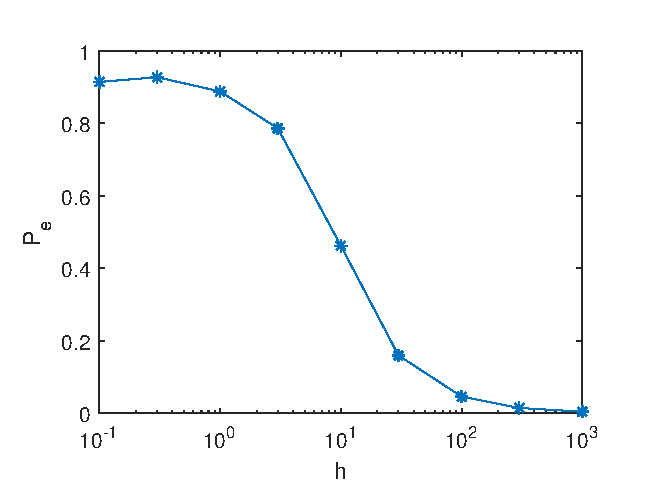
\includegraphics[width=0.33\linewidth]{F8he}}
\subfloat[corner]{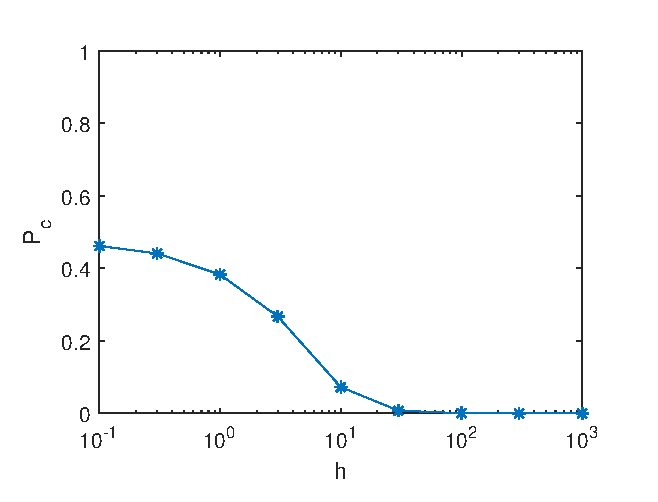
\includegraphics[width=0.33\linewidth]{F8hc}}
\caption{The degree of localization to the boundary varies to $h$ (parameter $p=0.5, K=10^3$)}
\label{fig:8h}
\end{figure}


\paragraph{relation of parameter p}

The degree of localization to the boundary varies to $p$ with parameter $h=1, K=10^3$ is shown in the Figure \ref{fig:8p}. {\color{red} unfinished, how to explain this result?}

\begin{figure}[h]
\centering
\subfloat[boundary]{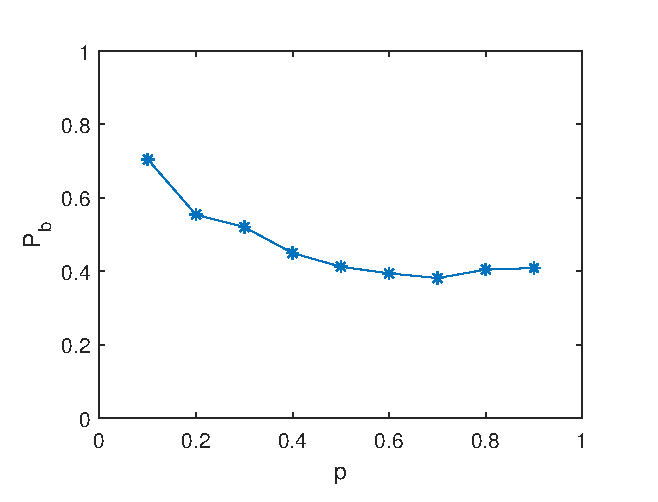
\includegraphics[width=0.33\linewidth]{F8pb}}
\subfloat[edge]{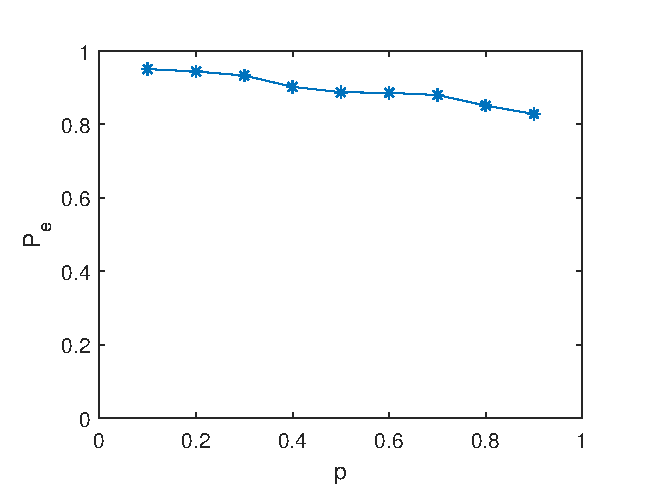
\includegraphics[width=0.33\linewidth]{F8pe}}
\subfloat[corner]{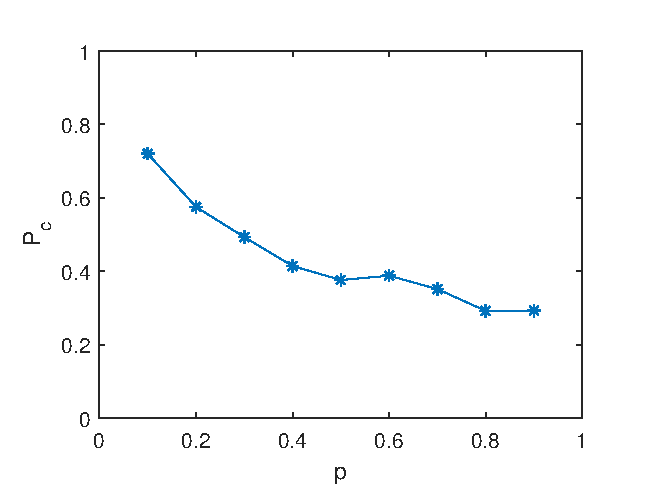
\includegraphics[width=0.33\linewidth]{F8pc}}
\caption{The degree of localization to the boundary varies to $p$ (parameter $h=1, K=10^3$)}
\label{fig:8p}
\end{figure}


\paragraph{relation of parameter K}

The degree of localization to the boundary varies to $K$ with parameter $p=0.5, h=1$ is shown in the Figure \ref{fig:8k}. {\color{red} unfinished, how to explain this result?}

\begin{figure}[h]
\centering
\subfloat[boundary]{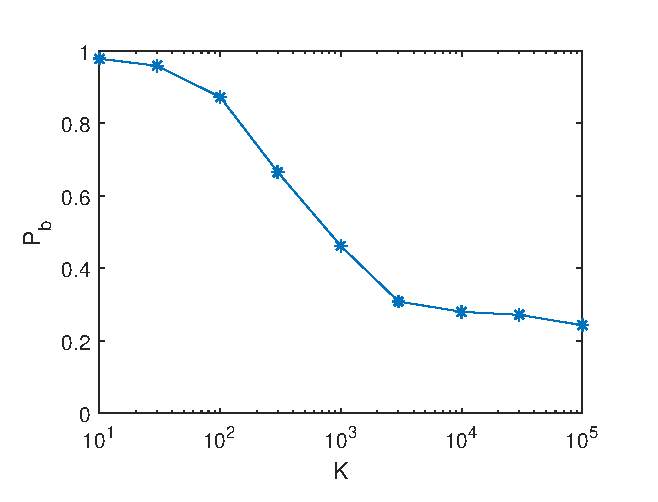
\includegraphics[width=0.33\linewidth]{F8kb}}
\subfloat[edge]{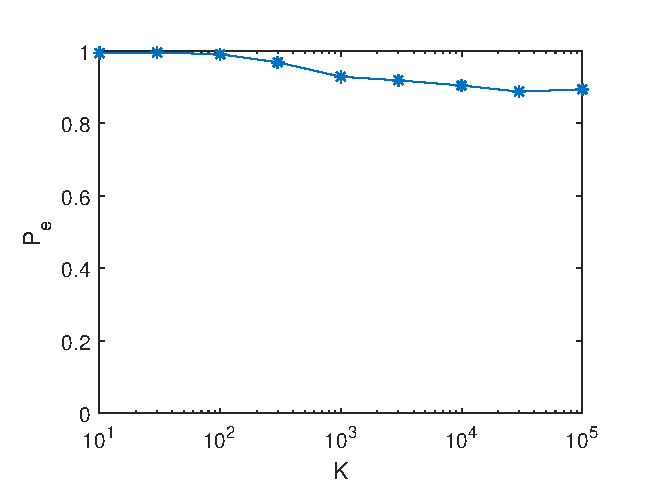
\includegraphics[width=0.33\linewidth]{F8ke}}
\subfloat[corner]{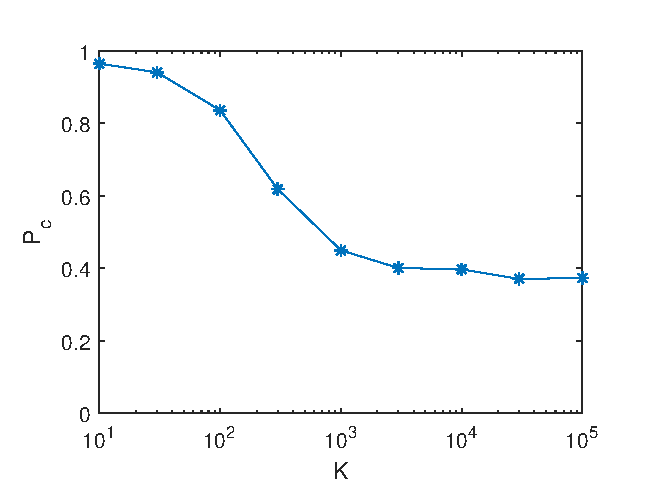
\includegraphics[width=0.33\linewidth]{F8kc}}
\caption{The degree of localization to the boundary varies to $K$ (parameter $p=0.5, h=1$)}
\label{fig:8k}
\end{figure}

\subsection{A theoretical result for 1-d case}

In 1-d case, for Dirhclet BC, the first eigenmode will localize to the longest interval on which $V(x) = 0$. Noting that there is some symmetric properties in Neumann BC. As shown in Figure \ref{fig:BC}, for an interval with left Neumann BC and right Dirichlet BC, the smallest eigenvalue is equal to the smallest eigenvalue on an interval with twice length and Dirichlet BC. Then we can get, if the longest extended subdomian is near the boundary, the first eigenmode will localize to the boundary.

\begin{figure}[h]
\centering
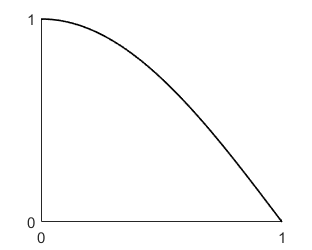
\includegraphics[height=0.15\textheight]{DN}
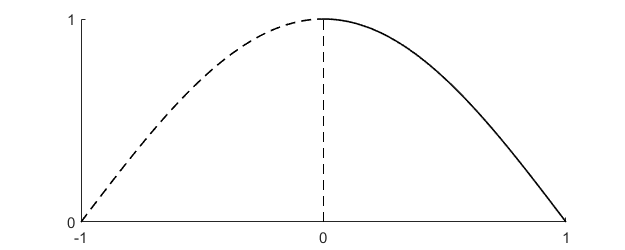
\includegraphics[height=0.15\textheight]{DD}
\caption{Extention for 1-d case}
\label{fig:BC}
\end{figure}

As shown in Figure \ref{fig:BC2}, we can also apply the theroy to 2-d case, in particular, the sub area near the corner will be extended twice. After extended, area of extended subdomains near the boundary become larger, that is for Neumann BC, eigenmodes are more likely localize to the boundary.

\begin{figure}[h]
\centering
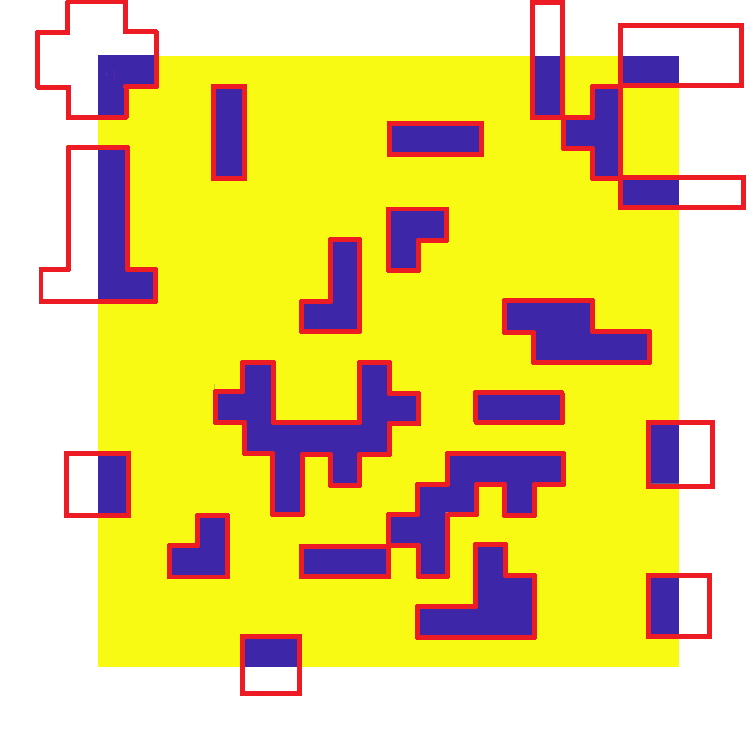
\includegraphics[width=0.33\linewidth]{BC2}
\caption{Extention in 2-d case. Blue for $V(x) = 0$ and yellow for $V(x) = K$. Effective subdomains are surronded by red lines.}
\label{fig:BC2}
\end{figure}

For sufficient big $K$ and small $h$, the probability of "the first eigenmode localize to the boundary" is equal to the probability of the event that "the longest extended subdomain locates on the boundary". We can get its probability is
\begin{align}\label{eq:bdprob}
P_b = q^2 p^2 \sum_{k=1}^{\infty} q^{k-2} \sum_{n=1}^{k-1} (1 - q^{2 \max\{k-n,n\}-1})^{M-2} + p q^2 \sum_{n=1}^{\infty} (1 - p^{2 n-1})^{M-2} p^{n-1}
\end{align}

Figure \ref{fig:9} show the simulation results and theoretical predictions. We choose parameters $K = 5 \times 10^4, h = 0.01$. The whole domain is divieded into $N = 50$ intervals. The theoretical prediction is in good agreement with the simulation.
\begin{figure}[h]
\centering
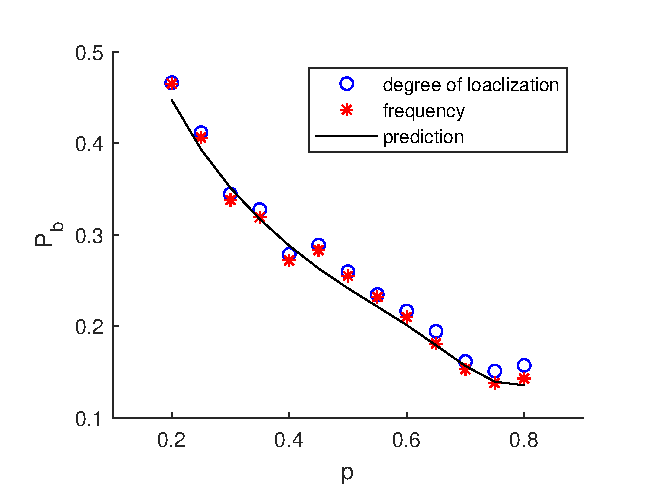
\includegraphics[width=0.33\linewidth]{F9}
\caption{Simulation results and theoretical predictions for large $K$ and small $h$. Blue circles represents the simulation result of $P_b$, red stars represents the frequency of the event "the longest extended subdomain locates on the boundary" in the simulation, black line represents the thoretical prediction of $P_b$ for different $p$.}
\label{fig:9}
\end{figure}

\section{Multimodality}\label{sec:multimodality}

Firstly, we introduce a simple example. Consider eigenmodes of pootential shown in Figure \ref{fig:10e}(a) with Dirichlet BC. Due to the symmetric properties of the potential, we have double eigenvalue $\lambda_1 = \lambda_2 = 211.5469$ and any linear combination ofeigenmode 1 and eigenmode 2 is also an eigenmmode.

Noting that both first and second eigenmodes have two peaks which called multimodality. From Figure \ref{fig:10e}(c) we can see, one can hardly get information of multimodality from the landscape. Landscape can only tell us where eigenmodes might localize, but can not describe the multimodality.

\begin{figure}[h]
\centering
\subfloat[potential]{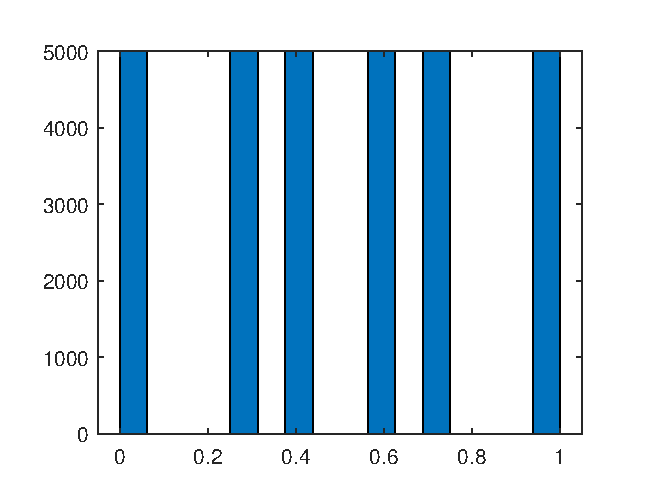
\includegraphics[width=0.33\linewidth]{F10EP}}
\subfloat[eigenmode]{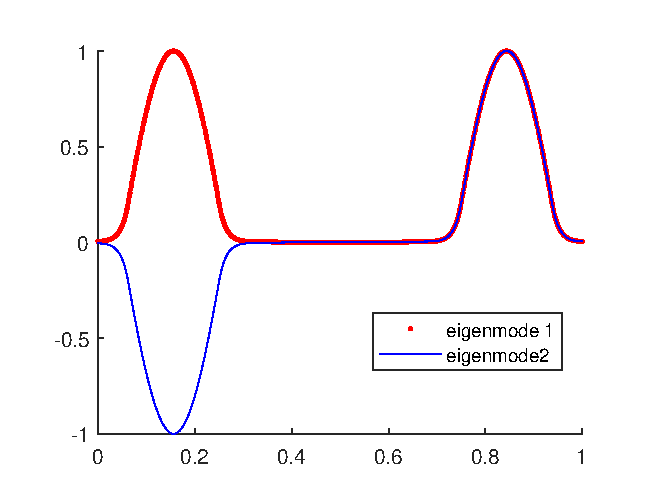
\includegraphics[width=0.33\linewidth]{F10EU}}
\subfloat[landscape]{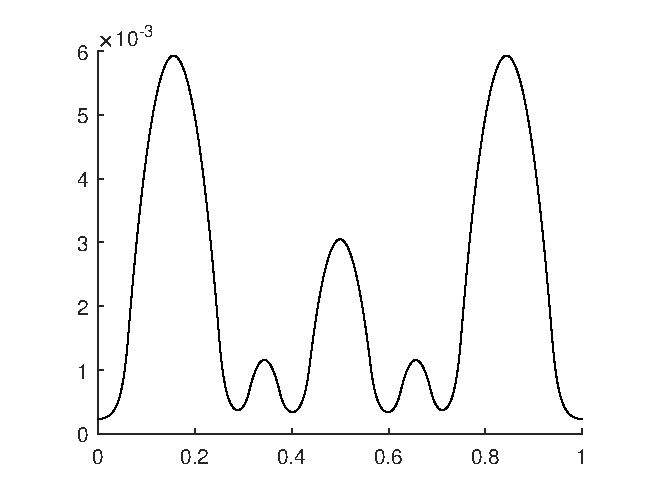
\includegraphics[width=0.33\linewidth]{F10EL}}
\caption{(a) The random potential $V(x)$ entering the equation($K = 8000$). (b) first 2 eigenmodes. (c) corresponding valleyline.}
\label{fig:10e}
\end{figure}

Multimodality may appear when the first eigenvalue is equal to the second. Recall the analysis in Section \ref{sec:probability}, for sufficient large $K$, the probability of multimodality is equal to the probability of "the longest two extended subdomain are the same length". For Dirichlet BC, we can get its probability is
\begin{align}\label{eq:multiD}
P_D = 1 - p \sum_{n=1}^{\infty} (1 - p^{n-1})^{M-2} q^{n-1}
\end{align}
and for Neumann BC
\begin{align}\label{eq:multiN}
\begin{split}
P_N = 1 - & q^2 (M-2) \sum_{n=1}^{\infty} (1 - q^{(n-1)/2})^2 (1 - q^{n-1})^{M-3} q^{n-1} p \\
- & 2 q^2 \sum_{n=1}^{\infty} (1 - q^{2n-1})^{M-2} (1 - q^{n-1}) q^{n-1} p \\
- & 2 p q (M-1) \sum_{n=1}^{\infty} (1 - q^{(n-1)/2}) (1 - q^{n-1})^{M-2} q^{n-1} p \\
- & 2 p q \sum_{n=1}^{\infty} (1 - q^{2n-1})^{M-1} q^{n-1} p \\
- & p^2 M \sum_{n=1}^{\infty} (1 - p^{n-1})^{M-1} q^{n-1} p
\end{split}
\end{align}

Affected by calculation error, we can hardly observe that eigenvalues are exactly equal in practice, so we think that the multimodellity appears when the relative error between the first and the second eigenvalue satisity $\frac{\lambda_2 - \lambda_1}{\lambda_1} < 0.02$.


Figure \ref{fig:10} show the simulation results and theoretical predictions. We choose parameters $K = 3 \times 10^6$. The whole domain is divieded into $N = 50$ intervals. The theoretical prediction is in good agreement with the simulation.
\begin{figure}[h]
\centering
\subfloat[Dirichlet BC]{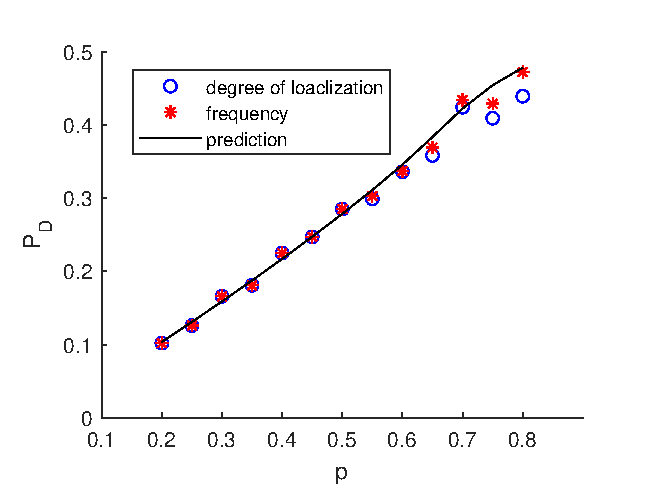
\includegraphics[width=0.33\linewidth]{F10D}}
\subfloat[Neumann BC]{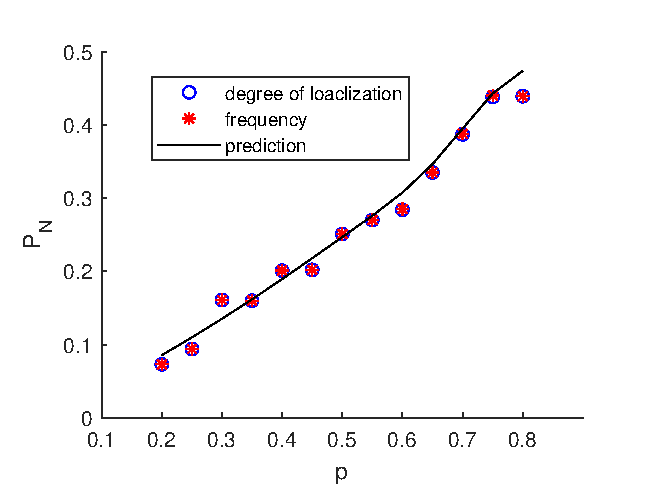
\includegraphics[width=0.33\linewidth]{F10N}}
\caption{Simulation results and theoretical predictions for large $K$. Blue circles represents the simulation result of $P_D$ and $P_N$, red stars represents the frequency of the event in the simulation, black lines represents the thoretical prediction of $P_D$ and $P_N$ for different $p$.}
\label{fig:10}
\end{figure}

\section{Phase transition}\label{sec:phase}

Consider 1-d case with parabolic BC, potietial is choosen as follows. As shown in Figure \ref{fig:11p}, in the whole domain $[0,1]$, the values of potential are $0$ and $K$ alternately in the intervals with length $L_2/2, L_1, L_2, L_3, L_4, L_3, L_2/2$. We can consider the potential as two wells $\Omega_1, \Omega_2$ with length $L_1$ and $2 L_3$, while there is a barrier with length $L_4$ in the middle of the second well.

\begin{figure}[h]
\centering
\includegraphics[width=0.7\linewidth]{PV}
\caption{A diagram of potential $V(x)$}
\label{fig:11p}
\end{figure}

In the potential, $L_2$ is big enough to seprate two wells and $L_4$ is small. For detials, potential must satisify: $L_3 < L_1 < 2 L_3$ (two wells are about the same length), $L_4 < L_3 / 2$ (barrier should be short enough), $L_2 > L_1+ L_3 + L_4 + L_3$ ($L_2$ should be big enough to seperate the two wells), and total length $L_1 + 2 L_2 + 2L_3 + L_4 = 1$.

Since the second well is longer, when $K$ is small, barrier is not strong enough, so the first eigenmode will localize to the second well. But when $K$ is big, the first eigenmode will localize to the first well. For increasing $K$, eigenmode will jump from the second well to the first, which is called phase transition.

We choose $L_1 = 1/12, L_2 = 2/5, L_3= 1/20, L_4 = 1/60$. The first two eigenmodes and landscapes for different $K$ is shown in Figure \ref{fig:12}. One can see that for different $K$, landscapes are almost same, but the eigenmodes changes a lot.
\begin{figure}[h]
\centering
\subfloat[eigenmode 1]{\includegraphics[width=0.3\linewidth]{F12U1}}
\subfloat[eigenmode 2]{\includegraphics[width=0.3\linewidth]{F12U2}}
\subfloat[landscape]{\includegraphics[width=0.3\linewidth]{F12W}}
\caption{The first two eigenmodes and landscapes for different $K$}
\label{fig:12}
\end{figure}

Eigenmodes and landscapes may appear two peakes in $\Omega_1$ and $\Omega_2$. For a certain function $u(x)$, we define the relative height of the left peak $F$ as 
\begin{align}
F = \frac{\max_{x \in \Omega_1} |u(x)|}{\max_{x \in \Omega_1} |u(x)| + \max_{x \in \Omega_2} |u(x)|}
\end{align}
Relative height of left peak in eigenmodes and landscapes are shown in Figure \ref{fig:12f} (a-c). one can see that the relative heigth of peak of landscape is approximately constant for different $K$ but eigenmodes appears phase transition. We define the $K$ satisify the left and right peak of the first eigenmode is equal in height as the critical point $K_c$ in phase transition.
\begin{figure}[h]
\centering
\subfloat[eigenmode 1]{\includegraphics[width=0.3\linewidth]{F12FU1}}
\subfloat[eigenmode 2]{\includegraphics[width=0.3\linewidth]{F12FU2}}
\subfloat[landscape]{\includegraphics[width=0.3\linewidth]{F12FW}}
\caption{Relative heights of peaks in eigenmodes and landscape various with parameter $K$.}
\label{fig:12f}
\end{figure}

%More simulation ressults in Tabel \ref{tab:1}.

Figure \ref{fig:12d} (b) shows the variation of the first and second eigenvalue with $K$. In this problem, the potential has two wells. So we can divide the problem into two subsystems. The eigenmode localized to the left corresponds to an subsystem, and the eigenmode localized to the left corresponds to another.

As shown in Figure \ref{fig:11a}, set the value in $\Omega_1$ to $K$ and we can get $V_1(x)$. Similiarly, set the value in $\Omega_2$ to $K$ and we can get $V_2(x)$. The system into two subsystems with potential $V_1(x)$ and $V_2(x)$.
\begin{figure}[h]
\centering
\subfloat[$V_1(x)$]{\includegraphics[width=0.49\linewidth]{PV1}}
\subfloat[$V_2(x)$]{\includegraphics[width=0.49\linewidth]{PV2}}
\caption{A diagram of potential $V_1(x)$ and $V_2(x)$ in subsystems.}
\label{fig:11a}
\end{figure}

We choose $L_1 = 1/12, L_2 = 2/5, L_3= 1/20, L_4 = 1/60$, the eigenmodes and eigenvalues of subsystems are shown in Figure \ref{fig:12d}. From Figure \ref{fig:12d} (a) we can see that eigenmodes of subsystems are almost same with the eigenmodes of the original problem. Figure \ref{fig:12d} shows the eigenvalues for different $K$. Both the first eigenvalues increase with the increase of K, but they increase at different rates. When one eigenvalue is equal to the other, the minimum eigenvalue changes from one to the other, then the phase transition occurs.
\begin{figure}[h]
\centering
\subfloat[eigenmodes]{\includegraphics[width=0.4\linewidth]{F12D1}}
\subfloat[eigenvalues]{\includegraphics[width=0.4\linewidth]{F12D2}}
\caption{Eigenmodes and eigenvalues of subsystems}
\label{fig:12d}
\end{figure}

We can proof that for parameter $K$, the first eigenvalue of subsystem on $\Omega_1$ satisify the equation
\begin{align}\label{eq:phase1}
0 = D_1(K, \lambda) = \alpha \tan(\alpha x_0) - \beta \tanh(\beta (\frac12 - x_0))
\end{align}
where $\alpha = \sqrt{\lambda}, \beta = \sqrt{K - \lambda}, x_0 = L_1 / 2$.

Similarly, the first eigenvalue of subsystem on $\Omega_1$ satisify the equation
\begin{align}\label{eq:phase2}
\begin{split}
0 = D_2(K, \lambda) = & (\alpha^2 - \beta^2)(\mathrm{e}^{2 \beta x_2} + \mathrm{e}^{2 \beta (x_1+x_3)}) / (\mathrm{e}^{2 \beta (x_1+x_3)} - \mathrm{e}^{2 \beta x_2}) \\
+ & (\alpha^2 + \beta^2)(\mathrm{e}^{2 \beta x_3} + \mathrm{e}^{2 \beta (x_1+x_2)}) / (\mathrm{e}^{2 \beta (x_1+x_3)} - \mathrm{e}^{2 \beta x_2}) \\
+ & 2 \alpha \beta \cot(\alpha (x_1 - x_2))
\end{split}
\end{align}
where $x_1 = L_4 / 2, x_2 = L_4 / 2 + L_3, x_3 = 1 / 2$.

When pahse transition occurs, eigenvalue in both subsystem are equal, so the citical point $K_c$ and the ciritcal eigenvalue $\lambda_c$ satisify
\begin{align}\label{eq:phase}
D_1(K_c, \lambda_c) = 0 \\
D_2(K_c, \lambda_c) = 0
\end{align}

We generate $L_1, L_2, L_3, L_4$ randomly, Firgure \ref{fig:13} shows the prediction from \ref{eq:phase} and the simulation results, we can see that the prediction is accurate.
\begin{figure}[h]
\centering
\subfloat[$K_c$]{\includegraphics[width=0.4\linewidth]{DfK}}
\subfloat[$\lambda_c$]{\includegraphics[width=0.4\linewidth]{Dfl}}
\caption{simulation and prediction results. x-axis reresents the prediction value and y-axis represents the simulation  results. Each blue point represents a random sample and the red line is $x=y$.}
\label{fig:13}
\end{figure}

%这里的4个变量,一共有3个自由度。我们选取要拟合的变量为
%$$ L_2 = \frac{N_2}{N_1 + 2 N_2 + N_3 + N_4 + N_5}, \quad L_4 = \frac{N_4}{N_3 + N_5}, \quad L_1 = \frac{N_1}{N_3 + N_5} $$
%\textbf{在拟合其中一个时,保持其余变量不变}。
%
%\subsection*{$L_2$和$K_c$之间的关系}
%
%$N_2$对应的区域,作用就是把两段区域分割开。相变的本质是子区域的特征值哪个更大,整个问题是定义在$[0,1]$上的,因此增加$L_2$相当于压缩两个子区域的区间长度,而区间长度的平方是和特征值成反比的。
%
%根据这些分析,我们猜测关系为
%$$ \frac{1}{K_c} = A_c (1 - 2 L_2)^2 $$
%
%在以下三组参数对模型进行拟合,得到拟合的参数值和$R^2$如下:
%\begin{align*}
%N=(5, n, 3, 1, 3), \quad n \in [20, 40] \quad A_c = 0.0345, \quad R^2 = 1 - 1.4 \times 10^{-7} \quad \text{图中紫色} \\
%N=(6, n, 4, 1, 4), \quad n \in [20, 40], \quad A_c = 0.0137, \quad R^2 = 1 - 5.9 \times 10^{-11} \quad \text{图中红色} \\
%N=(7, n, 5, 1, 5), \quad n \in [20, 40], \quad A_c = 0.0077, \quad R^2 = 1 - 1.1 \times 10^{-9} \quad \text{图中蓝色}
%\end{align*}
%由于数据是由模拟生成的,而不是从实际测量中获得,所以几乎没有什么误差,$R^2$的值十分接近1也是可以接受的。
%
%图\ref{fn2}中可以看出,拟合结果很好,这些直线都通过原点。$A_c$是一个和$L_2$无关的量,它越大代表相变点越小。
%\begin{figure}[h]
%\centering
%\includegraphics[width=0.4\linewidth]{L2Kc}
%\caption{拟合结果。横轴:$(1-2L_2)^2$,纵轴:$K_c$}
%\label{fn2}
%\end{figure}
%
%
%\subsection*{$L_4$和$A_c$之间的关系}
%
%进一步分析发现,如果$N_4$等于$0$,模型中就不会出现相变。在$N_4$靠近0的时候,相变点会不断变大,直到无穷,此时$A_c$趋于0,所以模型一定要过原点。
%
%我们猜测$L_4$和$A_c$之间的关系为
%$$ A_c = B_c L_4 $$
%
%在$N_4$很大的时候,相变会消失,也就是随着$L_4$的增大,$1/K_c$会在某个有限的位置趋于无穷。因此这里得到的关系只有在$L_4$较小的某个范围内才成立。
%
%在以下三组参数对模型进行拟合,得到拟合的参数值和$R^2$如下:
%\begin{align*}
%N=(5, 2(11+n), 3, n, 3), \quad n \in [0.4, 1.6], \quad B_c = 0.0129, \quad R^2 = 1 - 1.4 \times 10^{-3} \quad \text{图中紫色} \\
%N=(6, 2(14+n), 4, n, 4), \quad n \in [0.4, 1.8], \quad B_c = 0.0071, \quad R^2 = 1 - 8.6 \times 10^{-4} \quad \text{图中红色} \\
%N=(7, 2(17+n), 5, n, 5), \quad n \in [0.4, 2.1], \quad B_c = 0.0052, \quad R^2 = 1 - 1.2 \times 10^{-3} \quad \text{图中蓝色}
%\end{align*}
%
%图\ref{fn4}中可以看出,拟合结果比较好。
%\begin{figure}[h]
%\centering
%\includegraphics[width=0.4\linewidth]{L4Ac}
%\caption{拟合结果。横轴:$L_4$,纵轴:$A_c$}
%\label{fn4}
%\end{figure}
%
%\subsection*{$L_1$和$B_c$之间的关系}
%
%进一步分析发现,如果$N_1$等于$\max\{N_3,N_5\}$,模型中就不会出现相变。在$N_1$趋近于$\max\{N_3,N_5\}$的时候,相变点会不断变大,直到无穷,此时$B_c$趋于0,所以模型一定要过原点。
%
%同样的,随着$L_1$的增大,$1/K_c$会在某个有限的位置趋于无穷。因此这里得到的关系只有在$L_1$较小时成立。
%
%我们猜测在$0.5 < L_1 < 0.75$区间内,它和$K_c$之间的关系为
%$$ \log(B_c) = D_c (L_1 - 0.5) + E_c $$
%这个模型既不过原点,也不在有限点处趋于无穷,但是它是目前区间内和数据拟合效果最好的模型。
%
%在以下三组参数对模型进行拟合,得到拟合的参数值和$R^2$如下:
%\begin{align*}
%N=(n, 2(7+n), 3, 1, 3), \quad n \in [3.5, 4.5], \quad D_c = 7.3358, \quad E_c = -4.0118, \quad R^2 = 1 - 0.0024 \quad \text{图中紫色} \\
%N=(n, 2(9+n), 4, 1, 4), \quad n \in [4.5, 6.0], \quad D_c = 7.7312, \quad E_c = -4.1023, \quad R^2 = 1 - 0.006 \quad \text{图中红色} \\
%N=(n, 2(11+n), 5, 1, 5), \quad n \in [5.5, 7.5], \quad D_c = 8.0747, \quad E_c = -4.1830, \quad R^2 = 1 - 0.010 \quad \text{图中蓝色}
%\end{align*}
%
%图\ref{fn1}中可以看出,拟合结果比较好。由于已经消除了前两个变量的影响,这里的线看起来是重合的。
%\begin{figure}[h]
%\centering
%\includegraphics[width=0.4\linewidth]{L1Bc}
%\caption{拟合结果。横轴:$L_1 - 0.5$,纵轴:$\log(B_c)$}
%\label{fn1}
%\end{figure}
%
%\subsection*{总结}
%
%综上所述,得到总的公式为
%$$ \frac{1}{K_c} = (1-2L_2)^2 L_4 e^{D_c(L_1 - 0.5) - E_c} $$
%
%在一定范围内取很多点,验证公式的准确性。各项参数的范围是:
%\begin{align*}
%N_3 & \in [3, 6], \\
%N_1 & \in [N3+0.5, 1.5 N3],\\
%N_4 & \in [0.5, N_3/2], \\
%N_2 & \in [2(N_1+N_3+N_4+N_3), 3(N_1+N_3+N_4+N_3)]
%\end{align*}
%
%图\ref{fna}中可以看出,拟合结果比较好,预测值和实际值大致相等。(图中取$D_c=7.1, E_c=4$)
%\begin{figure}[h]
%\centering
%\includegraphics[width=0.4\linewidth]{LaKc}
%\caption{拟合结果。横轴:$\frac{1}{K_c}$预测值,纵轴:$\frac{1}{K_c}$模拟值,红线为直线$x=y$}
%\label{fna}
%\end{figure}

\section{Couclusion}

{\color{red} unfinished...}

\begin{appendices}

\section{Proof of landscape theorem \ref{th:landscape}}

Define the second order elliptic operator
\begin{align*}
\mathcal{L} u = -\nabla(A \nabla u) + b \cdot \nabla u + c u
\end{align*}
then $\lambda$, $u(x)$ and $w(x)$ satisify
\begin{align*}
\mathcal{L} u = \lambda u \qquad \mathcal{L} (\lambda w) = \lambda
\end{align*}

Noting that $u(x)$ can be seen as the solution of
\begin{align*}
\mathcal{L} u = g
\end{align*}
where $g(x) = \lambda u(x)$. Since $\|u\|_{\infty} = 1$, we have $g(x) \leq \lambda$.

According to the maximum principle, we can get
\begin{align*}
u(x) \leq \lambda \, w(x) \qquad x \in \Omega
\end{align*}

\section{Proof of theorem \ref{th:largeK}}

{\color{red} unfinished...}

\section{Geometric distributation approximation}

Accordong to the symmetric in Nuemann BC, for sufficient big K, the probability of "the first eigenmode localize to the boundary" is equal to the probability of the event that "twice of the length of a segment with value of 0 on the boundary is larger than all of segments with value of 0 inside".

Suppose that the previous two intervals with the value of $1$ and $0$, let the number of following intervals with the value of $0$ be $X$, then $X$ is a random variable. For a sufficient large $N$, $X$ approximately obeys the geometric distribution with parameter $p$.
$$ \mathbb{P}(X = n) = q^{n-1} p $$
thus
$$ \mathbb{P}(X < n) = 1 - q^{n-1} $$
where $q = 1 - p$.

Similarly, length of continuous intervals with of value $1$ is a random variable with probability
$$ \mathbb{P}(Y = n) = p^{n-1} q $$

In the whole interval, $X$ and $Y$ must appear alternately. The average length of each period is $E(X+Y) = \frac{1}{p q}$. So the average number of periods in the whole domain is $M = N p q$. In the average sense, we can approximately regard the whole domain consists of intervals with length $X_1, Y_1, \cdots, X_M, Y_M$. For a sufficient large $N$, random variables $X_1, Y_1, \cdots, X_M, Y_M$ are approximately independent.

\subsection{Callculation of equation \ref{eq:bdprob}}

The event "localize to the boundary" can be splitted into the following situations:

\paragraph*{situation 1}
$V(0) = V(1) = 0$ with probability $q^2$.

Under such conditions, we have
\begin{align*}
  & \mathbb{P}(\max\{X_2, X_3, \cdots, X_{M-1}\} < 2 \max\{X_1, X_M\}) \\
= & \sum_{m,n=1}^{\infty} \mathbb{P}(\max\{X_2, X_3, \cdots, X_{M-1}\} < 2 \max\{m,  n\}) \mathbb{P}(X_1 = m) \mathbb{P}(X_M = n) \\
= & \sum_{m,n=1}^{\infty} [\mathbb{P}(X_k < 2 \max\{m,n\}) ]^{M-2} \mathbb{P}(X_1 = m) \mathbb{P}(X_M = n)\\
= & \sum_{m,n=1}^{\infty} (1 - q^{2 \max\{m,n\}-1})^{M-2} q^{m-1} p q^{n-1} p\\
= & \sum_{k=1}^{\infty} q^{k-2} p^2 \sum_{n=1}^{k-1} (1 - q^{2 \max\{k-n,n\}-1})^{M-2} 
\end{align*}

\paragraph*{situation 2}
$V(0) = 0, V(1) = 1$ with probability $p q$.

Under such conditions, we have
\begin{align*}
  & \mathbb{P}(\max\{X_2, X_3, \cdots, X_{M}\} < 2 X_1) \\
= & \sum_{n=1}^{\infty} \mathbb{P}(\max\{X_2, X_3, \cdots, X_{M-1}\} < 2 n) \mathbb{P}(X_1 = n) \\
= & \sum_{n=1}^{\infty} [\mathbb{P}(X_k < 2 n)]^{M-1} \mathbb{P}(X_1 = n)\\
= & q \sum_{n=1}^{\infty} (1 - p^{2 n-1})^{M-2} p^{n-1}
\end{align*}

\paragraph*{situation 3}
$V(0) = 1, V(1) = 0$ with probability $p q$, which can be calculated simillary to situation 2.

In summary, probability of localize to the boundary is
\begin{align*}
q^2 p^2 \sum_{k=1}^{\infty} q^{k-2} \sum_{n=1}^{k-1} (1 - q^{2 \max\{k-n,n\}-1})^{M-2} + p q^2 \sum_{n=1}^{\infty} (1 - p^{2 n-1})^{M-2} p^{n-1}
\end{align*}

\subsection{Calculation of equation \ref{eq:multiD}}

For Dirichlet Boundary, probability of "there is a unique longest subdomain with $V(x)=0$" is
\begin{align*}
  & \sum_{k=1}^{M} \mathbb{P}(\max\{X_1, X_2, \cdots, X_{k-1}, X_{k+1}, \cdots, X_{M}\} < X_k) \\
= & M \; \mathbb{P}(\max\{X_{2}, X_{3}, \cdots, X_{M}\} < X_1) \\
= & M \sum_{n=1}^{\infty} \mathbb{P}(\max\{X_2, X_3, \cdots, X_{M-1}\} < n) \mathbb{P}(X_1 = n) \\
= & M \sum_{n=1}^{\infty} [\mathbb{P}(X_k < n)]^{M-1} \mathbb{P}(X_1 = n)\\
= & M \sum_{n=1}^{\infty} (1 - p^{n-1})^{M-1} q^{n-1} p
\end{align*}

\subsection{Calculation of equation \ref{eq:multiN}}

For Neumann Boundary, probability of "there is a unique longest extended subdomain with $V(x)=0$" can be splitted into the following situations:

\paragraph*{situation 1}
$V(0) = V(1) = 0$ with probability $q^2$.

Under such conditions, we have
\begin{align*}
  & \sum_{k=2}^{M-1} \mathbb{P}(\max\{2 X_1, X_2, \cdots, X_{k-1}, X_{k+1}, \cdots, 2 X_{M}\} < X_k) \\
+ & \mathbb{P}(\max\{X_2, \cdots, X_{M-1}, 2 X_M\} < 2 X_1) \\
+ & \mathbb{P}(\max\{2 X_1, X_2, \cdots, X_{M-1}\} < 2 X_M) \\
= & (M-2) \mathbb{P}(\max\{2 X_1, X_3 \cdots, 2 X_{M}\} < X_2) \\
+ & 2 \mathbb{P}(\max\{X_2, \cdots, X_{M-1}, 2 X_M\} < 2 X_1) \\
= & (M-2) \sum_{n=1}^{\infty} \mathbb{P}(\max\{2 X_1, X_3 \cdots, 2 X_{M}\} < n) \mathbb{P}(X_2 = n) \\
+ & 2 \sum_{n=1}^{\infty} \mathbb{P}(\max\{X_2, \cdots, X_{M-1}, 2 X_M\} < 2 n) \mathbb{P}(X_1 = n) \\
= & (M-2) \sum_{n=1}^{\infty} [\mathbb{P}(2 X_k < n)]^2 [\mathbb{P}(X_k < n)]^{M-3} \mathbb{P}(X_2 = n) \\
+ & 2 \sum_{n=1}^{\infty} [\mathbb{P}(X_k < 2 n)]^{M-2} \mathbb{P}(X_k < n) \mathbb{P}(X_1 = n) \\
= & (M-2) \sum_{n=1}^{\infty} (1 - q^{(n-1)/2})^2 (1 - q^{n-1})^{M-3} q^{n-1} p \\
+ & 2 \sum_{n=1}^{\infty} (1 - q^{2n-1})^{M-2} (1 - q^{n-1}) q^{n-1} p
\end{align*}

\paragraph*{situation 2}
$V(0) = 0, V(1) = 1$ with probability $p q$.

Under such conditions, we have
\begin{align*}
  & \sum_{k=2}^{M} \mathbb{P}(\max\{2 X_1, X_2, \cdots, X_{k-1}, X_{k+1}, \cdots, X_{M}\} < X_k) \\
+ & \mathbb{P}(\max\{X_2, \cdots, X_{M-1}, X_M\} < 2 X_1) \\
= & (M-1) \mathbb{P}(\max\{2 X_1, X_3 \cdots, X_{M}\} < X_2) \\
+ & \mathbb{P}(\max\{X_2, \cdots, X_{M-1}, X_M\} < 2 X_1) \\
= & (M-1) \sum_{n=1}^{\infty} \mathbb{P}(\max\{2 X_1, X_3 \cdots, X_{M}\} < n) \mathbb{P}(X_2 = n) \\
+ & \sum_{n=1}^{\infty} \mathbb{P}(\max\{X_2, \cdots, X_{M-1}, X_M\} < 2 n) \mathbb{P}(X_1 = n) \\
= & (M-1) \sum_{n=1}^{\infty} \mathbb{P}(2 X_k < n) [\mathbb{P}(X_k < n)]^{M-2} \mathbb{P}(X_2 = n) \\
+ & \sum_{n=1}^{\infty} [\mathbb{P}(X_k < 2 n)]^{M-1} \mathbb{P}(X_1 = n) \\
= & (M-1) \sum_{n=1}^{\infty} (1 - q^{(n-1)/2}) (1 - q^{n-1})^{M-2} q^{n-1} p \\
+ & \sum_{n=1}^{\infty} (1 - q^{2n-1})^{M-1} q^{n-1} p
\end{align*}

\paragraph*{situation 3}
$V(0) = 1, V(1) = 0$ with probability $p q$, which can be calculated simillary to situation 2.

\paragraph*{situation 4}
$V(0) = 1, V(1) = 1$ with probability $p^2$, which can be calculated simillary to Dirichlet BC.

In summary, probability of multimodellity on Neumann BC is
\begin{align*}
P_N = 1 - & q^2 (M-1) \sum_{n=1}^{\infty} (1 - q^{(n-1)/2}) (1 - q^{n-1})^{M-2} q^{n-1} p \\
- & 2 q^2 \sum_{n=1}^{\infty} (1 - q^{2n-1})^{M-1} q^{n-1} p \\
- & 2 p q (M-1) \sum_{n=1}^{\infty} (1 - q^{(n-1)/2}) (1 - q^{n-1})^{M-2} q^{n-1} p \\
- & 2 p q \sum_{n=1}^{\infty} (1 - q^{2n-1})^{M-1} q^{n-1} p \\
- & p^2 M \sum_{n=1}^{\infty} (1 - p^{n-1})^{M-1} q^{n-1} p
\end{align*}

\section{Calculation of equation \ref{eq:phase1} and \ref{eq:phase2}}

As shown in the Figure \ref{fig:11b}, we can transform the problem into eigenvalue problem on a half interval with Neumann BC.

\begin{figure}[h]
\centering
\includegraphics[width=0.49\linewidth]{PV1a}
\includegraphics[width=0.49\linewidth]{PV2a}
\caption{A diagram of potential $V(x)$}
\label{fig:11b}
\end{figure}

\subsection*{subsystem on $\Omega_1$}

We can regard it as a problem with Neumann BC in $[0, 1/2]$. In the interval $[0, x_0]$, $V(x)$ takes the value $K$ and in $[x_0, 1/2]$ takes $0$, where $x_0 = L_1/2$.

We define $\alpha = \sqrt{\lambda}, \beta = \sqrt{K - \lambda}$. in the interval $[0, x_0]$, the eigenmode can be written as
\begin{align*}
u(x) = A \sin(\alpha x) + B \cos(\alpha x) \qquad u'(x) = A \alpha \cos(\alpha x) - B \alpha \sin(\alpha x)
\end{align*}
and in the interval $[x_0, 1/2]$,
\begin{align*}
u(x) = C \exp(\beta x) + D \exp(-\beta x) \qquad u'(x) = C \beta \exp(\beta x) - D \beta \exp(-\beta x)
\end{align*}
where $A ,B, C, D$ are the parameter to be determined.

According to the Neumann BC and continuity, we have
\begin{align*}
u'(0) & = A \alpha = 0 \\
u'(1/2) & = C \beta \exp(\beta/2) - D \beta \exp(-\beta/2) = 0 \\
u(x_0) & = A \sin(\alpha x_0) + B \cos(\alpha x_0) = C \exp(\beta x_0) + D \exp(-\beta x_0) \\
u'(x_0) & = A \alpha \cos(\alpha x_0) - B \alpha \sin(\alpha x_0) = C \beta \exp(\beta x_0) - D \beta \exp(-\beta x_0)
\end{align*}
that is
\begin{align*}
\left[\begin{array}{cccc} \alpha & 0 & 0 & 0\\ 0 & 0 & \beta \mathrm{e}^{\frac{\beta}{2}} & - \beta \mathrm{e}^{-\frac{\beta}{2}}\\ \sin\!\left(\alpha x_0\right) & \cos\!\left(\alpha x_0\right) & - \mathrm{e}^{\beta x_0} & - \mathrm{e}^{- \beta x_0}\\ \alpha \cos\!\left(\alpha x_0\right) & - \alpha \sin\!\left(\alpha x_0\right) & - \beta \mathrm{e}^{\beta x_0} & \beta \mathrm{e}^{- \beta x_0} \end{array}\right]
\left[\begin{array}{c} A \\ B \\ C \\ D \end{array}\right]
=
\left[\begin{array}{c} 0 \\ 0 \\ 0 \\ 0 \end{array}\right]
\end{align*}

The existence of solutions is equivalent to
\begin{align*}
\det(A) = \alpha \mathrm{e}^{2 \beta x_0} \sin\!\left(\alpha x_0\right) - \beta \mathrm{e}^{\beta} \cos\!\left(\alpha x_0\right) + \alpha \mathrm{e}^{\beta} \sin\!\left(\alpha x_0\right) + \beta \mathrm{e}^{2 \beta x_0} \cos\!\left(\alpha x_0\right) = 0
\end{align*}
that is
\begin{align*}
D_1(K, \lambda) = \alpha \tan(\alpha x_0) - \beta \tanh(\beta (\frac12 - x_0)) = 0
\end{align*}

\subsection*{subsystem on $\Omega_2$}

We can regard it as a problem with Neumann BC in $[0, 1/2]$. In the interval $[0, x_1]$ and $[x_2, 1/2]$, $V(x)$ takes the value $K$ and in $[x_1, x_2]$ takes $0$. Where $x_1 = L_4/2, x_2 = N_4/2 + N_3$.

In the interval $[0, x_0]$, the eigenmode can be written as
\begin{align*}
u(x) = A \exp(\beta x) + B \exp(-\beta x) \qquad u'(x) = A \beta \exp(\beta x) - B \beta \exp(-\beta x)
\end{align*}
and in the interval $[x_1, x_2]$,
\begin{align*}
u(x) = C \sin(\alpha x) + D \cos(\alpha x) \qquad u'(x) = C \alpha \cos(\alpha x) - D \alpha \sin(\alpha x)
\end{align*}
and in the interval $[x_2, 1/2]$,
\begin{align*}
u(x) = E \exp(\beta x) + F \exp(-\beta x) \qquad u'(x) = E \beta \exp(\beta x) - F \beta \exp(-\beta x)
\end{align*}
where $A ,B, C, D, E, F$ are the parameter to be determined.

According to the Neumann BC and continuity, we have
\begin{align*}
u'(0) & = A \beta - B \beta = 0 \\
u(x_1) & = A \exp(\beta x_1) + B \exp(-\beta x_1) = C \sin(\alpha x_1) + D \cos(\alpha x_1) \\
u'(x_1) & = A \beta \exp(\beta x_1) - B \beta \exp(-\beta x_1) = C \alpha \cos(\alpha x_1) - D \alpha \sin(\alpha x_1) \\
u(x_2) & = C \sin(\alpha x_2) + D \cos(\alpha x_2) = E \exp(\beta x_2) + F \exp(-\beta x_2) \\
u'(x_2) & = C \alpha \cos(\alpha x_2) - D \alpha \sin(\alpha x_2) = E \beta \exp(\beta x_2) - F \beta \exp(-\beta x_2) \\
u'(1/2) & = E \beta \exp(\beta/2) - F \beta \exp(-\beta/2) = 0
\end{align*}
that is
\begin{align*}
\left[\begin{array}{cccccc} 1 & -1 & 0 & 0 & 0 & 0\\ \mathrm{e}^{\beta x_1} & \mathrm{e}^{- \beta x_1} & - \sin\!\left(\alpha x_1\right) & - \cos\!\left(\alpha x_1\right) & 0 & 0\\ \beta \mathrm{e}^{\beta x_1} & - \beta \mathrm{e}^{- \beta x_1} & - \alpha \cos\!\left(\alpha x_1\right) & \alpha \sin\!\left(\alpha x_1\right) & 0 & 0\\ 0 & 0 & \sin\!\left(\alpha x_2\right) & \cos\!\left(\alpha x_2\right) & - \mathrm{e}^{\beta x_2} & - \mathrm{e}^{- \beta x_2}\\ 0 & 0 & \alpha \cos\!\left(\alpha x_2\right) & - \alpha \sin\!\left(\alpha x_2\right) & - \beta \mathrm{e}^{\beta x_2} & \beta \mathrm{e}^{- \beta x_2}\\ 0 & 0 & 0 & 0 & \mathrm{e}^{\frac{\beta}{2}} & - \mathrm{e}^{-\frac{\beta}{2}} \end{array}\right]
\end{align*}

The existence of solutions is equivalent to
\begin{align*}
& \alpha^2 \mathrm{e}^{2 \beta (x_{1} + x_{2})}  + \alpha^2 \mathrm{e}^{2 \beta (x_{1} + x_{3})} \\
+ & \beta^2 \mathrm{e}^{2 \beta (x_{1} + x_{2})} - \beta^2 \mathrm{e}^{2 \beta (x_{1} + x_{3})} \\
+ & \alpha^2 \mathrm{e}^{2 \beta x_{2}}  + \alpha^2 \mathrm{e}^{2 \beta x_{3}} \\
- & \beta^2 \mathrm{e}^{2 \beta x_{2}} + \beta^2 \mathrm{e}^{2 \beta x_{3}} \\
+ & 2 \alpha \beta \mathrm{e}^{2 \beta (x_{1} + x_{3})} \cot(\alpha (x_{1} - x_{2})) - 2 \alpha \beta \mathrm{e}^{2 \beta x_{2}} \cot(\alpha (x_{1} - x_{2})) = 0
\end{align*}

that is
\begin{align*}
0 = D_2(K, \lambda) = & (\alpha^2 - \beta^2)(\mathrm{e}^{2 \beta x_2} + \mathrm{e}^{2 \beta (x_1+x_3)}) / (\mathrm{e}^{2 \beta (x_1+x_3)} - \mathrm{e}^{2 \beta x_2}) \\
+ & (\alpha^2 + \beta^2)(\mathrm{e}^{2 \beta x_3} + \mathrm{e}^{2 \beta (x_1+x_2)}) / (\mathrm{e}^{2 \beta (x_1+x_3)} - \mathrm{e}^{2 \beta x_2}) \\
+ & 2 \alpha \beta \cot(\alpha (x_1 - x_2))
\end{align*}
where $x_3 = \frac12$.

\end{appendices}

\begin{thebibliography}{99} 
\bibitem{pnas} M. Filoche and S. Mayboroda. Universal mechanism for Anderson and weak localization, PNAS. vol. 109, no. 37, 14761–14766
\end{thebibliography}

\end{document}
